%======================================================================
% CHAPTER 5 — RELEASE 3: ARTIFICIAL INTELLIGENCE AND MACHINE LEARNING
%              (SPRINT 4)
% Methodology: CRISP-ML
% Content: ATB Customer Risk ML platform (Jupyter → XGBoost → MLflow → Streamlit)
% Skeleton aligned with supervisor-approved NotMyChapitre5.tex
%======================================================================
\chapter{Release 3: Artificial Intelligence and Machine Learning}
\label{chap:release3}

%----------------------------------------------------------------------
\section{Introduction}
%----------------------------------------------------------------------
Releases~1 and~2 of the ATB BI platform established a secure orchestration engine
(Apache Airflow), a Kimball constellation data warehouse, and an
interactive Streamlit decision dashboard driven by a transparent three-pillar rules
engine. \textbf{Release~3 --- Sprint~4} constitutes the qualitative leap from
\emph{descriptive} steering to \emph{predictive} intelligence: complementing the
auditable warehouse score with a supervised Machine Learning layer that screens
customers, surfaces disagreement alerts, and exposes model quality to risk managers
in real time.

This sprint delivers four interconnected innovations:
\begin{enumerate}
    \item \textbf{CRISP-ML lifecycle} applied end-to-end: from business understanding
          through Jupyter exploratory analysis, model engineering, MLflow tracking,
          and production deployment inside the existing dashboard shell.
    \item \textbf{XGBoost production classifier} trained on warehouse features
          (KYC, balances, sector, tenure) to predict $P(\text{high risk})$ where
          \texttt{high risk} $\equiv$ \texttt{global\_risk\_score} $\geq 50$.
    \item \textbf{Dual-layer risk architecture}: the rules engine remains the official
          auditable score; ML acts as a screening assistant that flags cases where
          model and rules diverge.
    \item \textbf{Operational integration}: nightly/weekly Airflow retraining,
          batch scoring into the \texttt{PFE\_ML} warehouse schema, and a
          five-tab \emph{ML Risk Intelligence} Streamlit module (live demo, batch
          alerts, curves \& SHAP, metrics, full predictor).
\end{enumerate}

Sprint~4 directly addresses User Stories US~10 to US~14 defined in
Chapter~2: train the algorithm, consult predictions, read curve interpretations,
compare risk by sector/zone, and export predictive scores.

%======================================================================
\section{Adoption of the CRISP-ML Methodology}
\label{sec:crispml_adoption}
%======================================================================

Global project governance remains \textbf{Scrum} (three-week sprints, prioritised
backlog, sprint reviews). For the AI/ML component of Sprint~4, this governance was
reinforced by \textbf{CRISP-ML} (\textit{Cross-Industry Standard Process for Machine
Learning}), the extension of CRISP-DM with explicit model-quality and deployment
phases already introduced in Chapter~1.

CRISP-ML provides three guarantees absent from an ad hoc notebook workflow:
\begin{itemize}
    \item \textbf{Full traceability}: every feature choice, hyperparameter, and
          performance threshold is logged in MLflow (\texttt{4\_ml/mlruns/}).
    \item \textbf{Integrated quality assurance}: acceptance gates (F1 $\geq 0.70$,
          ROC-AUC $\geq 0.80$) are defined \emph{before} declaring a model
          production-ready.
    \item \textbf{Reproducibility}: the pipeline is entirely scripted
          (\texttt{run\_training.py}, five ordered Jupyter notebooks); a
          \texttt{git pull} plus warehouse connection suffices to regenerate
          artefacts.
\end{itemize}

\subsection{The Six CRISP-ML Phases Applied to Sprint~4}

\begin{table}[H]
\centering
\caption{CRISP-ML phase mapping $\leftrightarrow$ Sprint~4 deliverables}
\label{tab:crispml-mapping-atb}
\begin{tabular}{|c|l|l|}
\hline
\textbf{Phase} & \textbf{CRISP-ML name} & \textbf{Sprint~4 deliverable} \\
\hline
1 & Business Understanding & Dual-layer rules + ML architecture (US~10--14) \\
2 & Data Understanding \& Preparation & 5 Jupyter notebooks + leakage-safe features \\
3 & Model Engineering & XGBoost + 3 baselines, SMOTETomek, MLflow runs \\
4 & Model Evaluation & ROC/PR, confusion matrix, SHAP, overfitting checks \\
5 & Model Deployment & Streamlit \emph{ML Risk Intelligence} + \emph{MLflow Registry} pages \\
6 & Monitoring \& Maintenance & Airflow \texttt{dag\_ml\_pipeline}, Docker, batch scoring \\
\hline
\end{tabular}
\end{table}
%======================================================================
\section{Business Understanding}
\label{sec:phase1_business}
%======================================================================

\subsection{Problem Statement and Objectives}

Phase~1 formalises the needs of ATB risk stakeholders \emph{before} any modelling.
Two complementary business challenges guided the architecture:

\begin{enumerate}
    \item \textbf{Instant high-risk screening}: compliance officers and branch risk
          managers must identify fragile profiles in seconds, not after a manual
          spreadsheet review.
    \item \textbf{Early warning beyond static rules}: the three-pillar warehouse
          score (\texttt{global\_risk\_score}) is explainable but rule-bound; ML
          must learn non-linear patterns (overdraft behaviour, stale KYC, salary
          pressure) that precede tier escalation.
\end{enumerate}

\subsection{Dual-Layer Decision Architecture}

Rather than replacing the GIMSI-validated rules engine, we designed a
\textbf{dual-layer} architecture where each layer has a distinct responsibility:

\begin{table}[H]
\centering
\caption{Dual-layer architecture --- roles and responsibilities}
\label{tab:dual-layer-roles}
\begin{tabular}{|l|p{5.2cm}|p{5.2cm}|}
\hline
\textbf{Dimension} & \textbf{Rules engine (DWH)} & \textbf{XGBoost ML} \\
\hline
Task & Deterministic 3-pillar scoring & Binary classification $P(\text{high risk})$ \\
Output & \texttt{global\_risk\_score} [0--100] + \texttt{risk\_tier} & Probability $\in [0,1]$ + label \\
Threshold & Fixed: score $\geq 50$ & Optimised on F1 (production $\approx 0.953$) \\
Inputs & Compliance / financial / behavioural indices & 34+ customer attributes (no score leakage) \\
Role & Official auditable score & Screening assistant + disagreement alerts \\
Usage & Regulatory reporting, KPI dashboards & On-demand in Streamlit + nightly batch \\
\hline
\end{tabular}
\end{table}

The Streamlit banner (\texttt{ml\_page.py}) makes this contract explicit to end
users: rules compute the official score; ML predicts high risk from attributes and
highlights cases requiring manual review when the two layers disagree.

\subsection{A Priori Acceptance Criteria (CRISP-ML Quality Gate)}

In line with CRISP-ML, acceptance thresholds were fixed \emph{before} the final
training run (documented in \texttt{FULL\_INTEGRATION\_STATUS.md}):
\begin{itemize}
    \item \textbf{F1 score} (test) $\geq 0.70$
    \item \textbf{ROC-AUC} (test) $\geq 0.80$
    \item \textbf{PR-AUC} monitored (critical given class imbalance $\approx 1.3\%$ positives)
    \item \textbf{Train--test F1 gap} $< 10\%$ (overfitting control)
    \item \textbf{No target leakage}: \texttt{global\_risk\_score}, pillar indices,
          and \texttt{risk\_tier} are explicitly excluded in
          \texttt{features.py}.
\end{itemize}

%======================================================================
\section{Data Understanding \& Preparation}
\label{sec:phase2_data}
%======================================================================

\subsection{Exploratory Data Analysis}

Before building any model, a five-notebook analysis pipeline was carried out
to understand the data, identify risks (such as class imbalance and target
leakage), and guide feature engineering choices.

\begin{table}[H]
\centering
\caption{Analysis notebook pipeline --- Sprint~4}
\label{tab:notebook-pipeline}
\begin{tabular}{|c|p{4cm}|p{7cm}|}
\hline
\textbf{\#} & \textbf{Notebook} & \textbf{Purpose} \\
\hline
01 & Data Profiling & Class balance, missing values, leakage audit \\
02 & Feature Engineering & Derived indicators, temporal train/test split \\
03 & Model Training & Four algorithms benchmarked and tracked \\
04 & SHAP Explainability & Global and local feature importance plots \\
05 & Model Selection & Final metric grid and production decision \\
\hline
\end{tabular}
\end{table}

\textbf{Data source.} The model is trained on customer records extracted from
the data warehouse, joining transaction facts with customer dimension attributes.
The full population contains 281{,}960 records, of which up to 5{,}000 are
sampled for iterative training runs.

\textbf{Binary target construction:}
\begin{equation}
\text{risk\_target} =
\begin{cases}
1 & \text{if } \texttt{global\_risk\_score} \geq 50 \quad (\text{high risk}) \\
0 & \text{otherwise}
\end{cases}
\label{eq:risk-target}
\end{equation}

\textbf{Class imbalance.} The exploratory analysis reveals a strongly imbalanced
target: only approximately \textbf{1.3\%} of customers are classified as high-risk.
This motivates the use of SMOTETomek resampling and prioritises F1 score, recall,
and PR-AUC over raw accuracy as evaluation criteria.

% --- SCREENSHOT: copy 4_ml/outputs/eda_target_and_distribution.png → figures/
\begin{figure}[H]
\centering
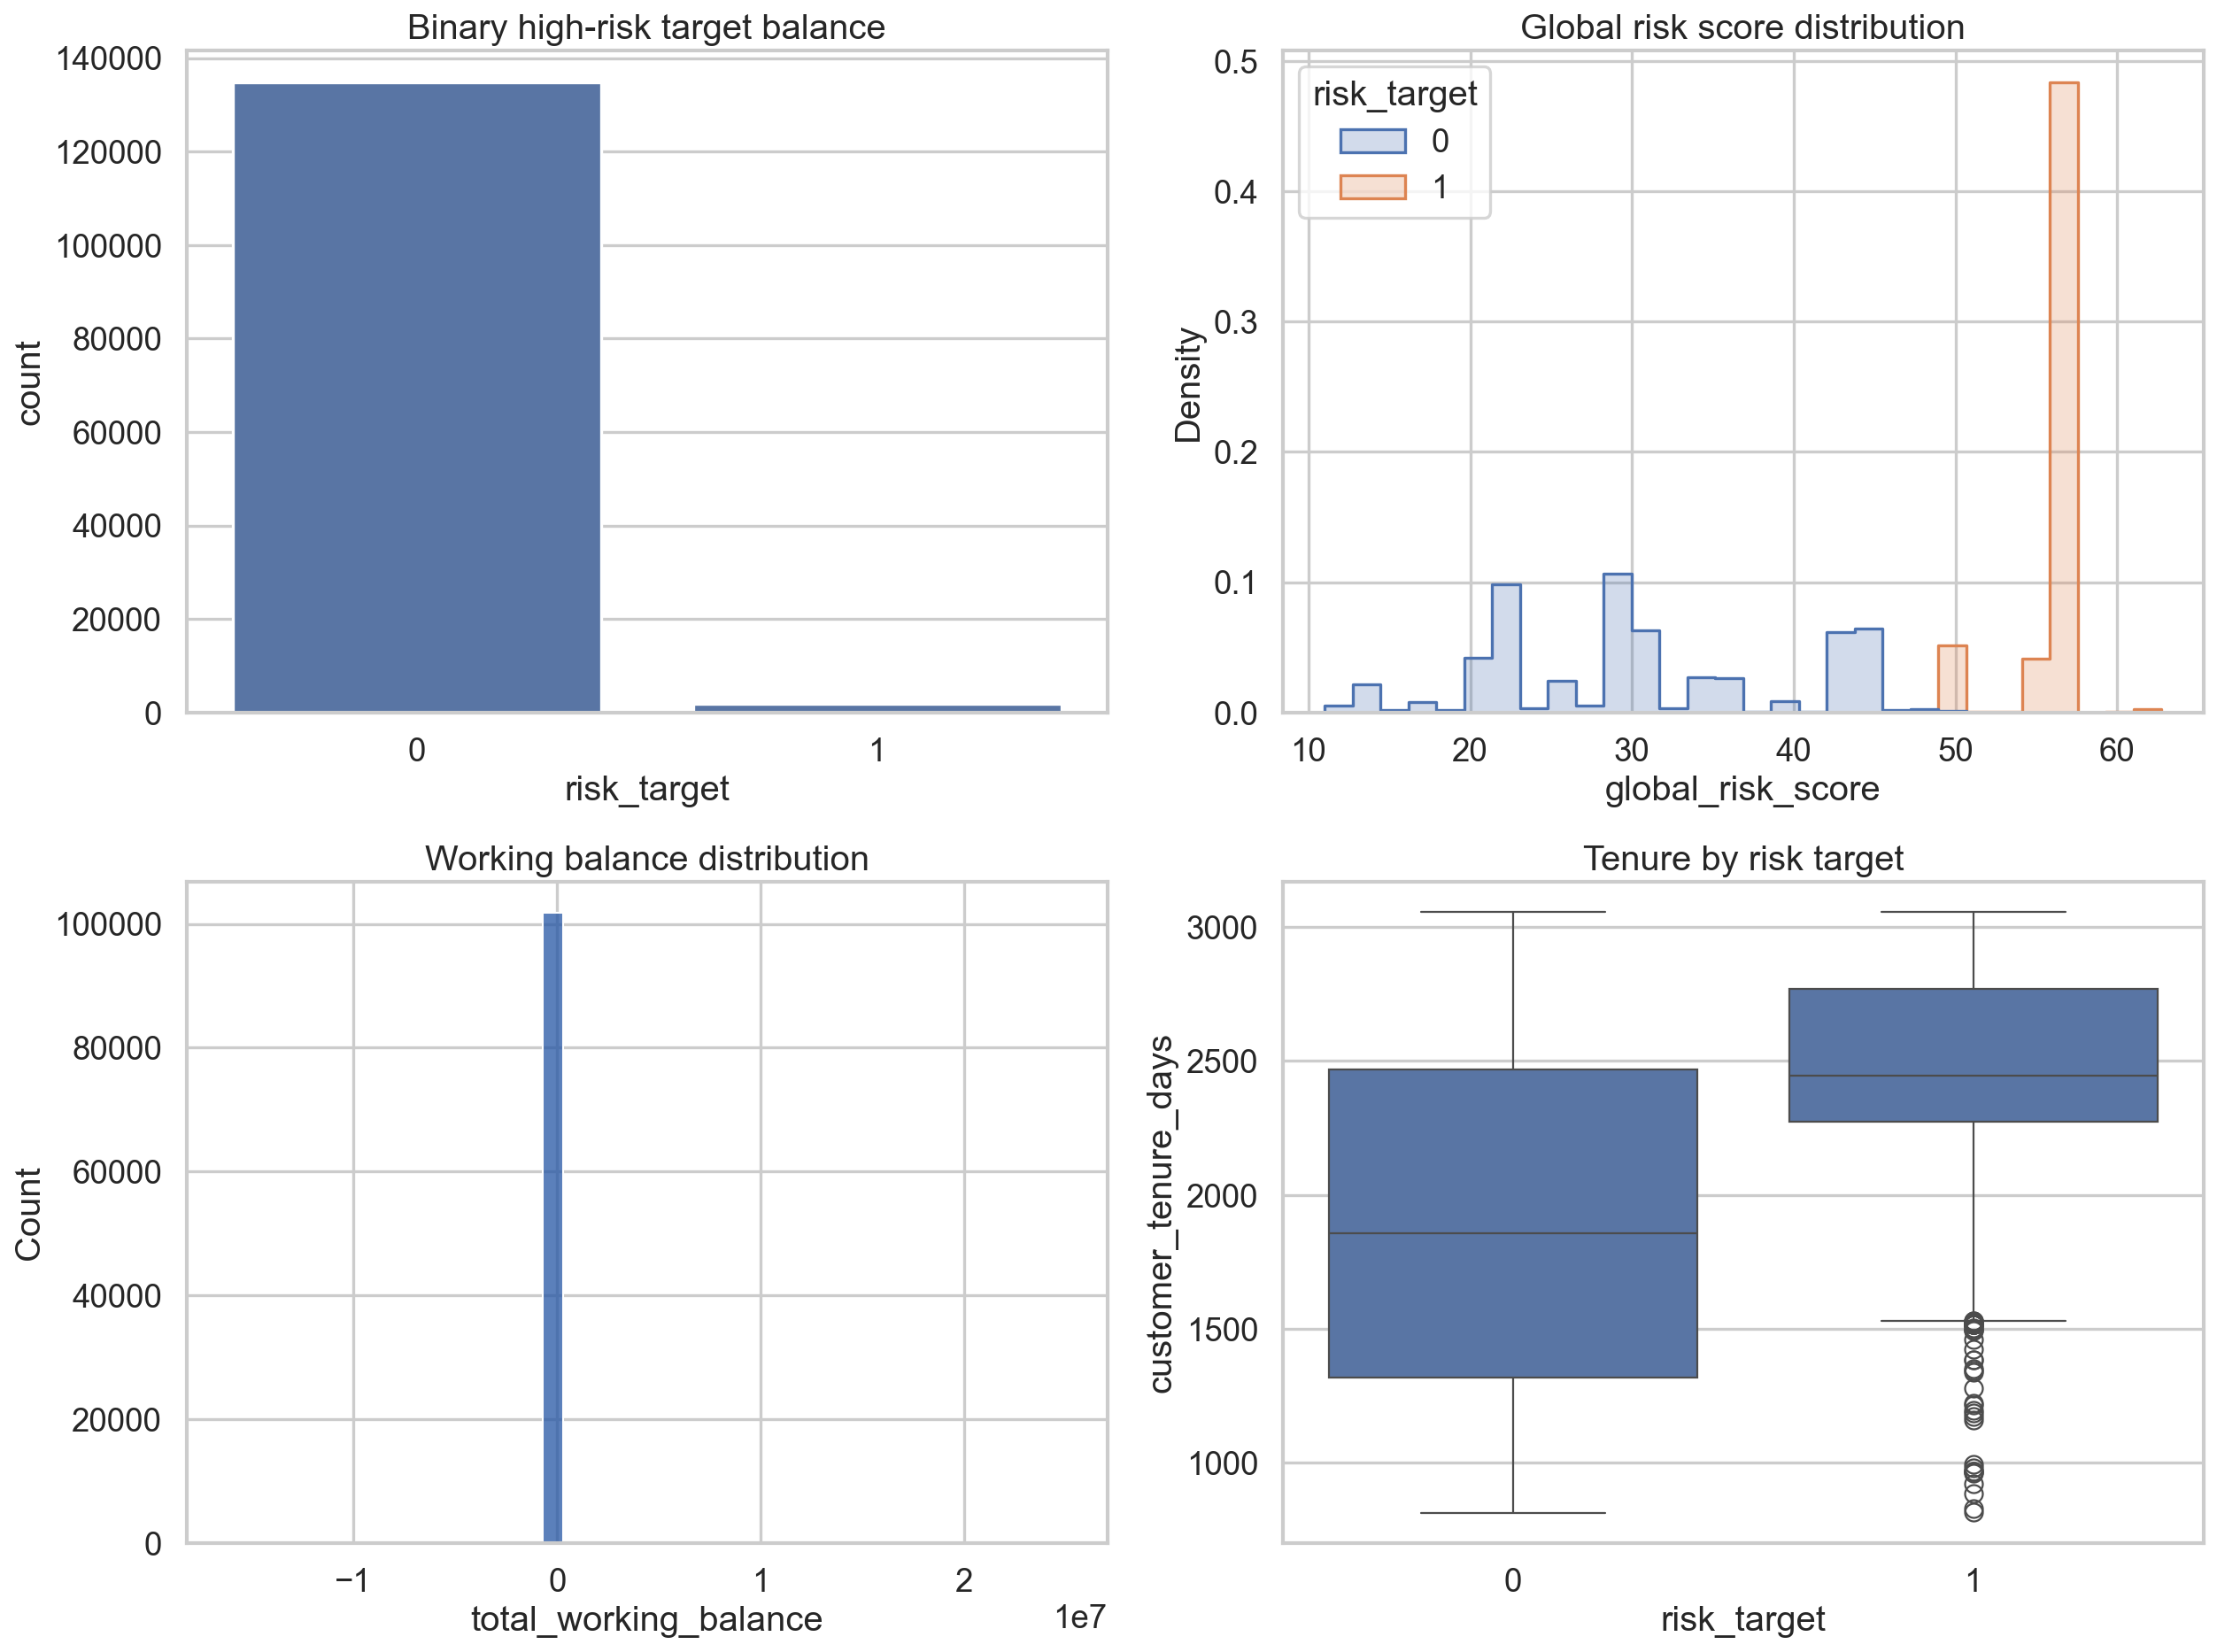
\includegraphics[width=0.75\textwidth]{figures/eda_target_and_distribution.png}
\caption{EDA distribution of global risk score and binary target balance}
\label{fig:eda-target-dist}
\end{figure}
\noindent The continuous GRS mass sits well below 50; the binary
cut at 50 yields only $\approx 1.3\%$ positives hence F1, recall and PR-AUC
dominate accuracy in later evaluation.

% --- SCREENSHOT: copy 4_ml/outputs/eda_correlation_heatmap.png → figures/
\begin{figure}[H]
\centering
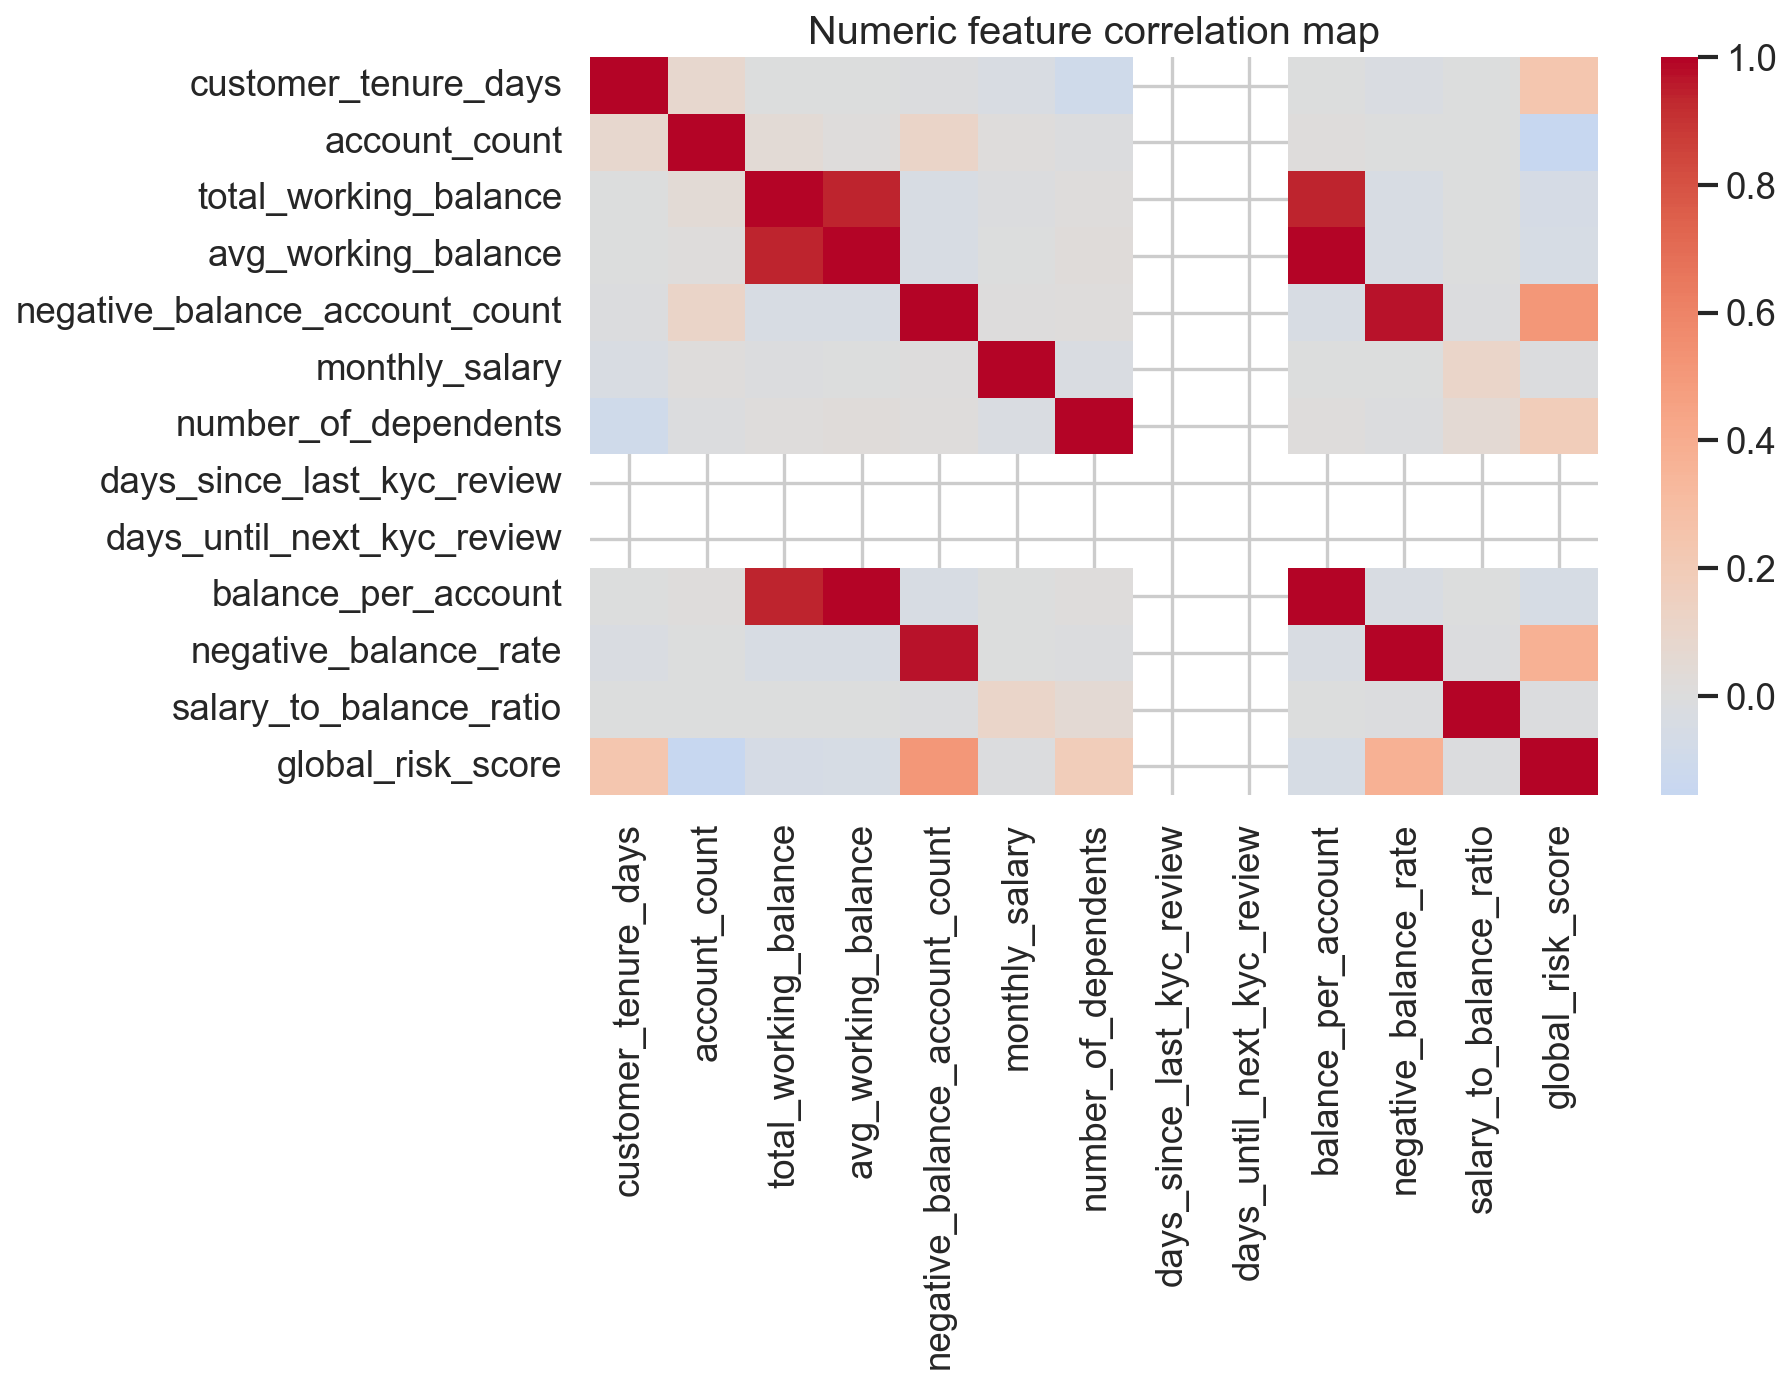
\includegraphics[width=0.75\textwidth]{figures/eda_correlation_heatmap.png}
\caption{EDA correlation heatmap of numeric risk drivers}
\label{fig:eda-corr}
\end{figure}
\noindent Weak linear correlations among demographics confirm
that tree ensembles are a better inductive bias than a purely linear separator.

Key EDA findings that shaped feature engineering:
\begin{itemize}
    \item \textbf{KYC staleness} is strongly associated with elevated compliance
          risk; customers with outdated identity records are more likely to appear
          in the high-risk class.
    \item \textbf{Financial stress signals} such as overdraft frequency and
          a high salary-to-balance ratio clearly separate the high-risk tail
          from the general population.
    \item \textbf{Low linear correlations} between raw demographic attributes
          confirm that tree-based, non-linear models are the most appropriate
          family for this classification task.
\end{itemize}

\subsection{Feature Engineering and Variable Selection}

A total of \textbf{34 input features} are fed to the model, organised into
three functional categories. To prevent \emph{target leakage}, the warehouse
risk score, its three component indices, and the risk tier label are
explicitly excluded from the feature set.

The engineered indicators below are computed from raw warehouse fields and
capture key dimensions of customer risk:

\begin{table}[H]
\centering
\caption{Engineered features and their business meaning}
\label{tab:engineered-features}
\begin{tabular}{|p{4.8cm}|l|p{5.5cm}|}
\hline
\textbf{Feature} & \textbf{Type} & \textbf{Business meaning} \\
\hline
Days since last KYC review & Numeric & Time elapsed since regulatory identity check \\
Has overdraft & Binary & Whether the customer holds any overdrawn account \\
Negative balance rate & Numeric & Share of accounts currently in negative balance \\
Salary-to-balance ratio & Numeric & Income relative to liquidity; signals financial pressure \\
KYC stale / very stale & Binary & Review overdue by more than 1 or 2 years \\
Is new customer & Binary & Tenure below 12 months \\
Balance per account & Numeric & Average balance across all held accounts \\
\hline
\end{tabular}
\end{table}

In addition, the model uses four \textbf{compliance flags} drawn directly
from the warehouse: KYC completeness status, politically exposed person (PEP)
status, a general compliance flag, and the presence of an active compliance
decision. Finally, \textbf{demographic and segmentation attributes} such as
employment status, gender, marital and residence status, branch area, sector,
industry, and customer segment are included, bringing the feature total to 34.

\subsection{Preprocessing Pipeline}

\begin{table}[H]
\centering
\caption{Preprocessing steps applied before model training}
\label{tab:preprocessing}
\begin{tabular}{|l|p{9cm}|}
\hline
\textbf{Step} & \textbf{Description} \\
\hline
Imputation & Median substitution for numeric fields; most-frequent value for categoricals \\
Encoding & One-hot encoding for all categorical variables; unknown categories ignored at inference \\
Scaling & Standard normalisation applied for Logistic Regression only \\
Class balancing & SMOTETomek applied after encoding, before classifier fitting \\
Temporal split & 80\% training / 20\% test, ordered chronologically to prevent data leakage \\
\hline
\end{tabular}
\end{table}

%======================================================================
\section{Model Engineering}
\label{sec:phase3_modeling}
%======================================================================

\subsection{Experiment Tracking with MLflow}

All training experiments are tracked using \textbf{MLflow}. Each algorithm
produces a separate logged run containing its hyperparameters, performance
metrics, and a serialised model artefact. The best-performing model is
registered under the name \texttt{Customer Risk Classifier } and
promoted to the \textbf{Production} stage, making it available to the
dashboard without any manual file handling.

\begin{figure}[H]
\centering
\resizebox{\linewidth}{!}{%
\begin{tikzpicture}[
  node distance=0.4cm and 0.8cm,
  every node/.style={font=\small},
  box/.style={rectangle, rounded corners=3pt, draw=black!60, fill=blue!8,
              minimum width=2.4cm, minimum height=0.75cm, align=center},
  arrow/.style={->, thick, draw=black!60},
  note/.style={font=\footnotesize\itshape, text width=2.4cm, align=center}
]
\node[box] (train) {Train};
\node[box, right=of train] (log) {Log run};
\node[box, right=of log] (reg) {Register};
\node[box, right=of reg] (prod) {Promote to\\Production};
\node[box, right=of prod] (score) {Batch score};

\draw[arrow] (train) -- (log);
\draw[arrow] (log) -- (reg);
\draw[arrow] (reg) -- (prod);
\draw[arrow] (prod) -- (score);

\node[note, below=0.2cm of train] {Hyperparameters\\+ metrics logged};
\node[note, below=0.2cm of log] {Run stored in\\MLflow experiment};
\node[note, below=0.2cm of reg] {Model registered\\with version tag};
\node[note, below=0.2cm of prod] {Previous version\\archived};
\node[note, below=0.2cm of score] {Predictions written\\to warehouse};
\end{tikzpicture}%
}
\caption{MLflow model lifecycle: from training run to warehouse-persisted predictions}
\label{fig:mlflow-lifecycle}
\end{figure}
\noindent Every experiment is a logged run; only the winning
artefact is registered, promoted to Production, then used for batch scoring.

\subsection{Benchmark: Four Supervised Classifiers}

Four classifiers were evaluated under identical conditions: same 34-feature input
set, same SMOTETomek-balanced training split, same stratified 2-fold
with F1 as the optimisation metric, and the same
temporal test holdout . Each run was
individually logged in MLflow so that artefacts, hyperparameters, and metrics
are fully reproducible.

\begin{table}[H]
\centering
\caption{Comprehensive four-model comparison test-set metrics}
\label{tab:all-models-comparison}
\renewcommand{\arraystretch}{1.25}
\begin{tabular}{|l|c|c|c|c|c|c|c|}
\hline
\textbf{Model} & \textbf{Accuracy} & \textbf{F1} & \textbf{Precision} & \textbf{Recall} & \textbf{ROC-AUC} & \textbf{PR-AUC} & \textbf{Brier} \\
\hline
\textbf{XGBoost} & \textbf{0.9988} & \textbf{0.9545} & 0.9130 & \textbf{1.0000} & \textbf{1.0000} & \textbf{1.0000} & \textbf{0.0013} \\
Random Forest & 0.9975 & 0.8947 & \textbf{1.0000} & 0.8095 & 0.9998 & 0.9908 & 0.0024 \\
Extra Trees & 0.9869 & 0.5333 & 0.8000 & 0.4000 & 0.9960 & 0.8200 & 0.0131 \\
Logistic Regression & 0.9931 & 0.7556 & 0.7083 & 0.8095 & 0.9977 & 0.8137 & 0.0065 \\
\hline
\end{tabular}
\end{table}

\textbf{Reading the table.}
\begin{itemize}
    \item \textbf{XGBoost} dominates on every metric that matters for imbalanced
          screening: F1 (+6.0 pp over Random Forest), perfect recall (zero missed
          high-risk cases), and a Brier score five times lower than Logistic Regression.
    \item \textbf{Random Forest} achieves perfect precision (no false alarms) but
          sacrifices recall (19\% of high-risk customers missed) unacceptable
          when the business objective is exhaustive screening.
    \item \textbf{Extra Trees} achieves high ROC-AUC yet collapses on F1 (0.53),
          reflecting an over-randomised structure that degrades recall at the
          production threshold. It was rejected despite passing the ROC gate.
    \item \textbf{Logistic Regression} provides a respectable linear baseline
          (F1 $= 0.76$) but cannot capture the non-linear interaction between
          PEP status, KYC staleness, and overdraft behaviour.
\end{itemize}

\subsection{Pairwise Analysis: XGBoost vs.\ Logistic Regression}

Logistic Regression is the natural interpretable baseline: it is fast, transparent,
and requires no hyperparameter tuning. However, it is limited to linear decision
boundaries and cannot capture compound risk patterns.

Test-set results:

\begin{table}[H]
\centering
\caption{Classification XGBoost vs.\ Logistic Regression (test set)}
\label{tab:xgb-vs-lr}
\begin{tabular}{|l|c|c|c|}
\hline
\textbf{Metric} & \textbf{XGBoost} & \textbf{Logistic Regression} & \textbf{Gain} \\
\hline
Accuracy & \textbf{0.9988} & 0.9931 & +0.6 pp \\
F1 & \textbf{0.9545} & 0.7556 & +19.9 pp \\
Precision & 0.9130 & 0.7083 & +20.5 pp \\
Recall & \textbf{1.0000} & 0.8095 & +19.1 pp \\
ROC-AUC & \textbf{1.0000} & 0.9977 & +0.2 pp \\
PR-AUC & \textbf{1.0000} & 0.8137 & +18.6 pp \\
Brier score & \textbf{0.0013} & 0.0065 & $-$80\% \\
\hline
\end{tabular}
\end{table}

XGBoost captures compound non-linear patterns (e.g.\ PEP status combined with
stale KYC and overdraft behaviour) that logistic weights cannot represent. The
F1 margin of \textbf{+19.9 pp} and a Brier score five times lower confirm that
XGBoost is the superior production choice.

% --- SCREENSHOT: copy 4_ml/outputs/03_model_comparison_bars.png
\begin{figure}[H]
\centering
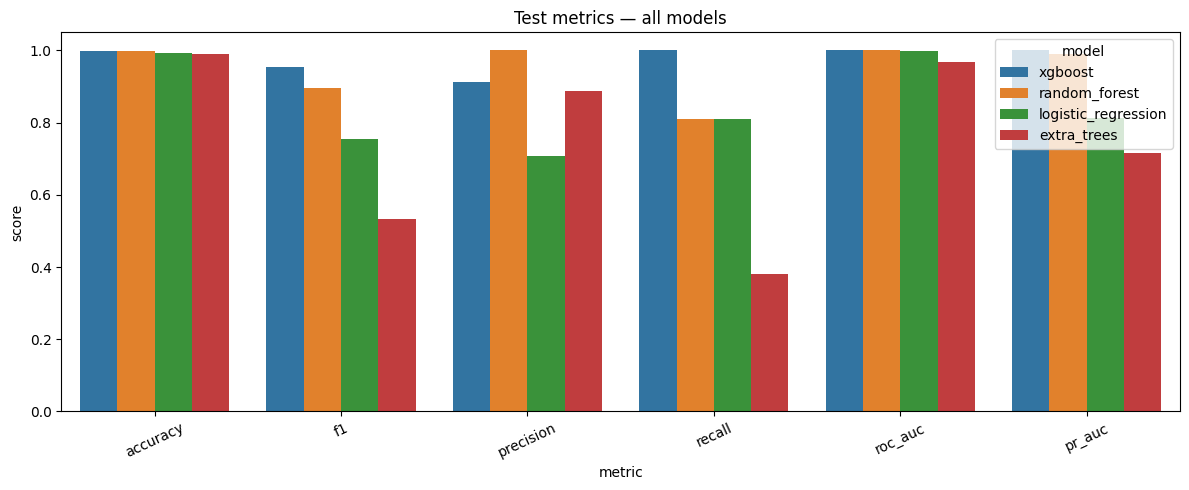
\includegraphics[width=0.92\textwidth]{figures/03_model_comparison_bars.png}
\caption{Bar chart comparing four algorithms on test F1 and ROC-AUC}
\label{fig:model-comparison-bars}
\end{figure}
\noindent Visual confirmation of Table~\ref{tab:all-models-comparison}:
XGBoost leads on F1 while all four models score high ROC-AUC --- F1 is therefore
the discriminating gate under imbalance.

\subsection{Pairwise Analysis: XGBoost vs.\ Random Forest}

\begin{table}[H]
\centering
\caption{Classification --- XGBoost vs.\ Random Forest (test set)}
\label{tab:xgb-vs-rf}
\begin{tabular}{|l|c|c|c|}
\hline
\textbf{Metric} & \textbf{XGBoost} & \textbf{Random Forest} & \textbf{Comment} \\
\hline
F1 & \textbf{0.9545} & 0.8947 & XGBoost +6.0 pp \\
Precision & 0.9130 & \textbf{1.0000} & RF more conservative on positives \\
Recall & \textbf{1.0000} & 0.8095 & XGBoost catches all test high-risk cases \\
ROC-AUC & \textbf{1.0000} & 0.9998 & Both excellent ranking \\
PR-AUC & \textbf{1.0000} & 0.9908 & Critical under 1.3\% prevalence \\
Optimal threshold & 0.953 & 0.612 & F1-optimised per model \\
\hline
\end{tabular}
\end{table}

Random Forest achieves perfect precision but sacrifices recall unacceptable
when the business goal is to \emph{screen} high-risk customers. XGBoost balances
both, meeting the quality gate with margin.

\subsection{Confusion Matrices}

The confusion matrices in Figure~\ref{fig:confusion-matrices} provide a direct
visual account of each model's classification behaviour on the held-out test
set. Each cell shows the count of true positives, true negatives, false positives,
and false negatives at each model's optimal threshold.

\begin{figure}[H]
\centering
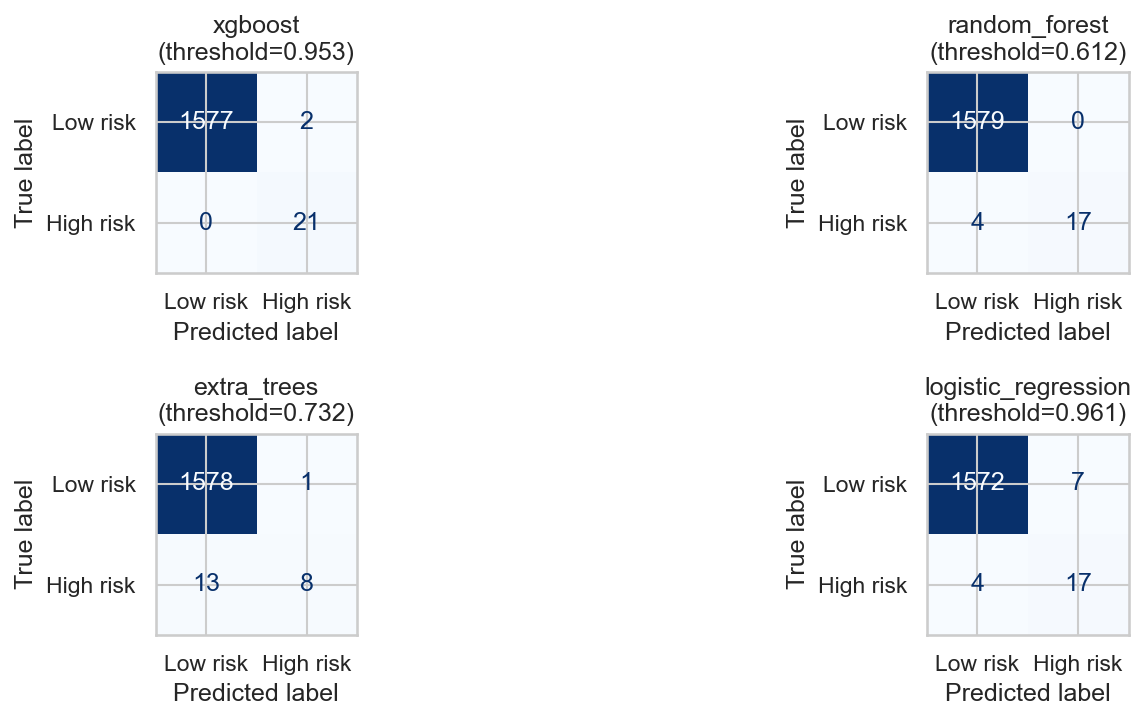
\includegraphics[width=0.95\textwidth]{figures/05_confusion_matrices.png}
\caption{Confusion matrices for all four classifiers at their respective
         optimal thresholds (XGBoost: 0.953; Random Forest: 0.612;
         Extra Trees: 0.732; Logistic Regression: 0.961). XGBoost is the
         only model with zero false negatives on the test set.}
\label{fig:confusion-matrices}
\end{figure}
\noindent XGBoost (top-left) recovers all 21 test high-risk
customers with only two false alarms; Random Forest trades recall for perfect
precision; Extra Trees collapses on false negatives.

\textbf{Reading the matrices.} XGBoost (top-left) correctly identifies all
21 high-risk customers in the test set with only 2 false alarms a false
negative count of zero. Random Forest (top-right) achieves zero false alarms
but misses 4 high-risk customers. Extra Trees (bottom-left) has the worst
recall, missing 13 out of 21 high-risk cases. Logistic Regression (bottom-right)
misses 4 cases, similar to Random Forest, but with 7 false alarms.

\subsection{Production Hyperparameters}

The XGBoost classifier is trained using gradient boosting with the binary
logistic objective. Hyperparameters including tree depth, learning rate, subsampling
rates, and regularisation terms are selected through randomised cross-validation
search optimising for F1. All settings are automatically logged to MLflow
for each training run.

The \textbf{decision threshold} is not fixed at the default value of 0.5.
Instead, it is selected from the precision--recall curve to maximise F1 on the
validation set, yielding a production threshold of $\approx 0.953$ for
XGBoost reflecting the model's high confidence distribution.

%======================================================================
\section{Model Evaluation}
\label{sec:phase4_evaluation}
%======================================================================

\subsection{Performance Synthesis vs.\ Acceptance Criteria}

\begin{table}[H]
\centering
\caption{Production XGBoost results vs.\ CRISP-ML quality gates}
\label{tab:perf-summary-atb}
\begin{tabular}{|l|c|c|c|}
\hline
\textbf{Criterion} & \textbf{Target} & \textbf{Result (test)} & \textbf{Status} \\
\hline
F1 score & $\geq 0.70$ & \textbf{0.9545} & \checkmark \\
ROC-AUC & $\geq 0.80$ & \textbf{1.0000} & \checkmark \\
PR-AUC & monitored & \textbf{1.0000} & \checkmark \\
Accuracy & informational & \textbf{0.9988} & \checkmark \\
Brier score & lower is better & \textbf{0.0013} & \checkmark \\
\hline
\end{tabular}
\end{table}

\textbf{All acceptance criteria are exceeded.} The model is declared
\textbf{production-ready} per CRISP-ML Phase~4.

\subsection{ROC, Precision--Recall, and Confusion Matrix}

Evaluation curves are generated during the training pipeline and reproduced
interactively in the dashboard's \textbf{Curves \& SHAP} tab, where the
threshold slider allows risk officers to explore the precision--recall
tradeoff in real time.

% --- SCREENSHOT: copy 4_ml/outputs/05_roc_pr_curves.png
\begin{figure}[H]
\centering
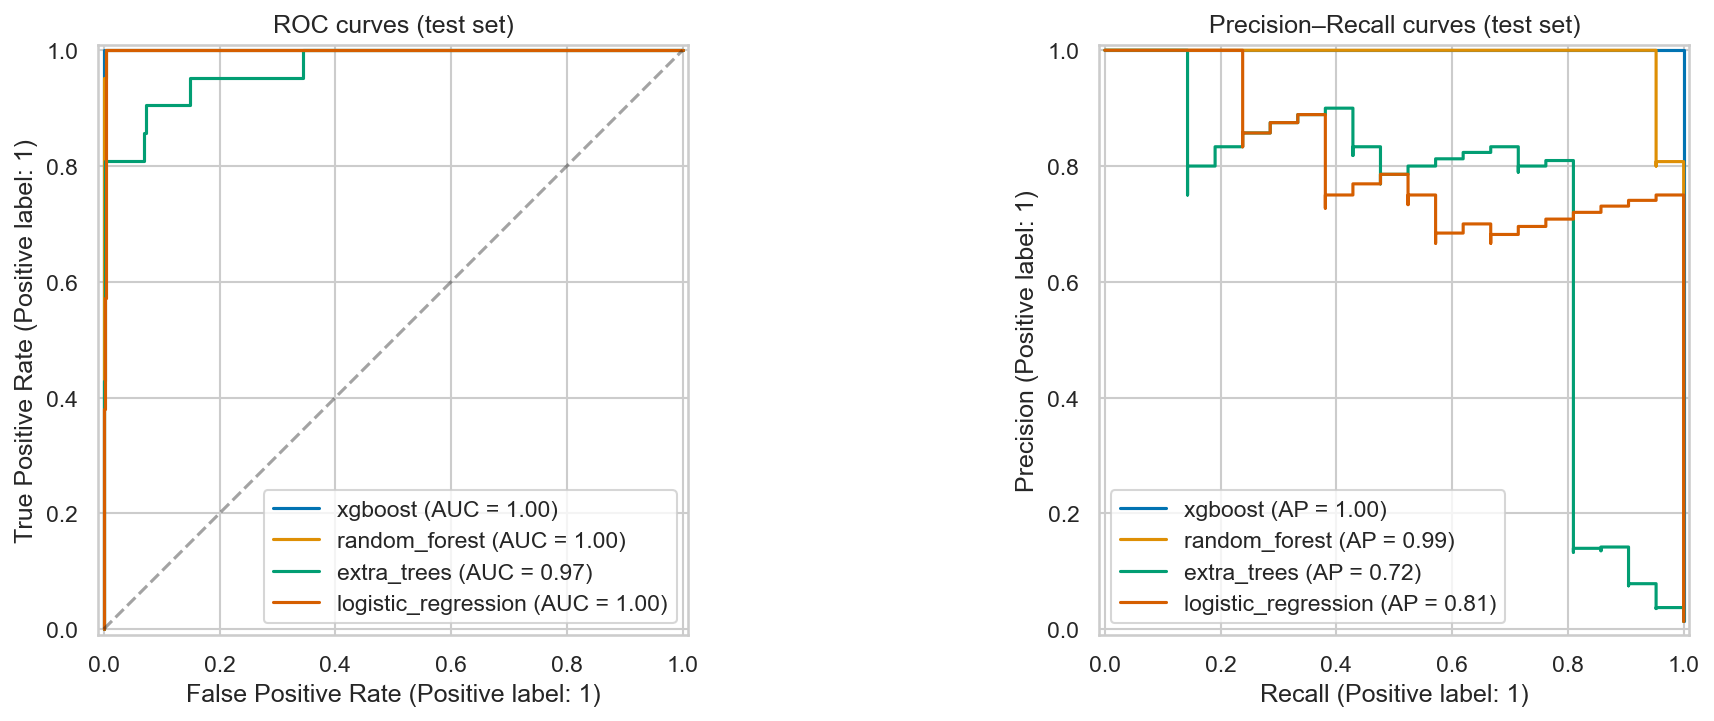
\includegraphics[width=0.92\textwidth]{figures/05_roc_pr_curves.png}
\caption{ROC and Precision--Recall curves XGBoost on test split }
\label{fig:roc-pr-notebook}
\end{figure}
\noindent Near-perfect ranking on both ROC and PR curves on the
temporal holdout; PR-AUC is the decisive view given the 1.3\% base rate.

% --- SCREENSHOT: Streamlit Curves & SHAP tab (live ROC/PR + confusion matrix)
\begin{figure}[H]
\centering
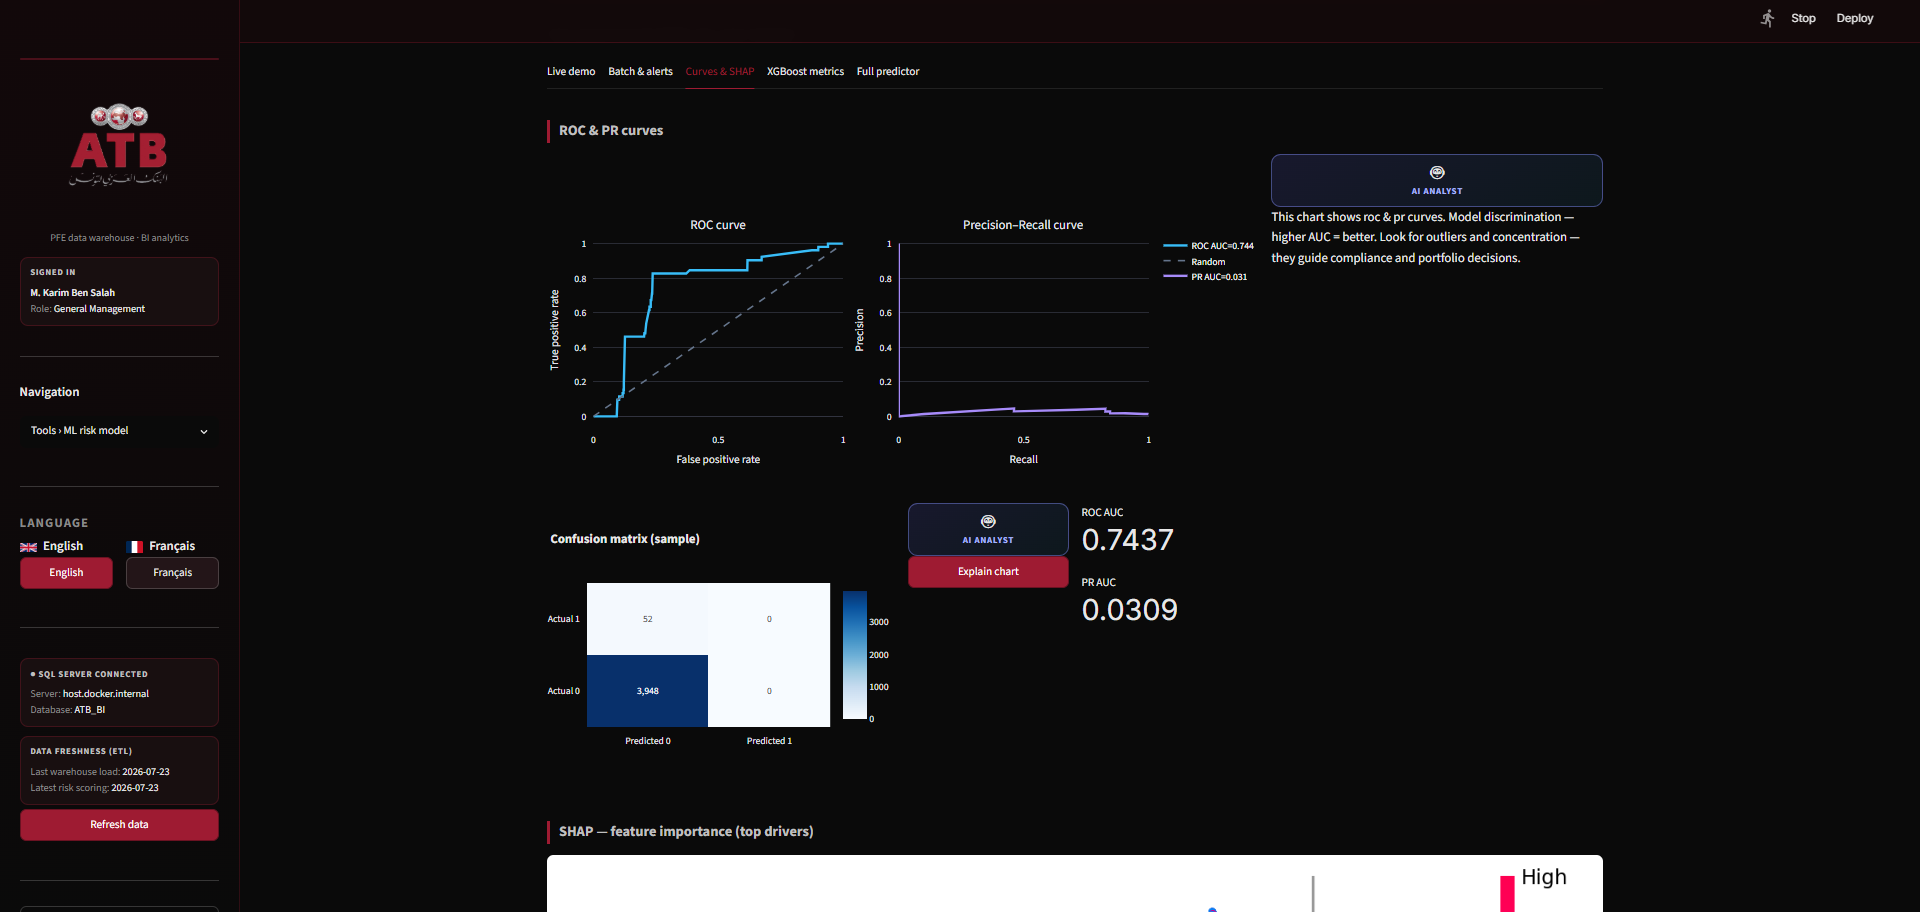
\includegraphics[width=0.95\textwidth]{figures/ml_curves_shap_tab.png}
\caption{Streamlit ML Risk Intelligence Page, \emph{Curves \& SHAP} tab with ROC-AUC and PR-AUC metrics}
\label{fig:streamlit-curves-shap}
\end{figure}
\noindent The same curves are interactive in production: officers
move the threshold slider and watch precision, recall and F1 update without
retraining.

At the production threshold, the confusion matrix on the held-out temporal test set
shows near-perfect separation. The dashboard additionally offers a
\textbf{threshold what-if slider}: precision, recall, and F1 are recomputed
instantly without retraining.

\subsection{Overfitting and Robustness}

The training pipeline compares train and test F1 scores for each algorithm.
The production XGBoost model maintains a well-controlled generalisation gap.
Extra Trees, by contrast, achieved strong training scores but collapsed to
F1 $= 0.53$ on the test set reflecting over-randomised trees that fail
to generalise and was rejected despite an acceptable ROC-AUC.

\begin{figure}[H]
\centering
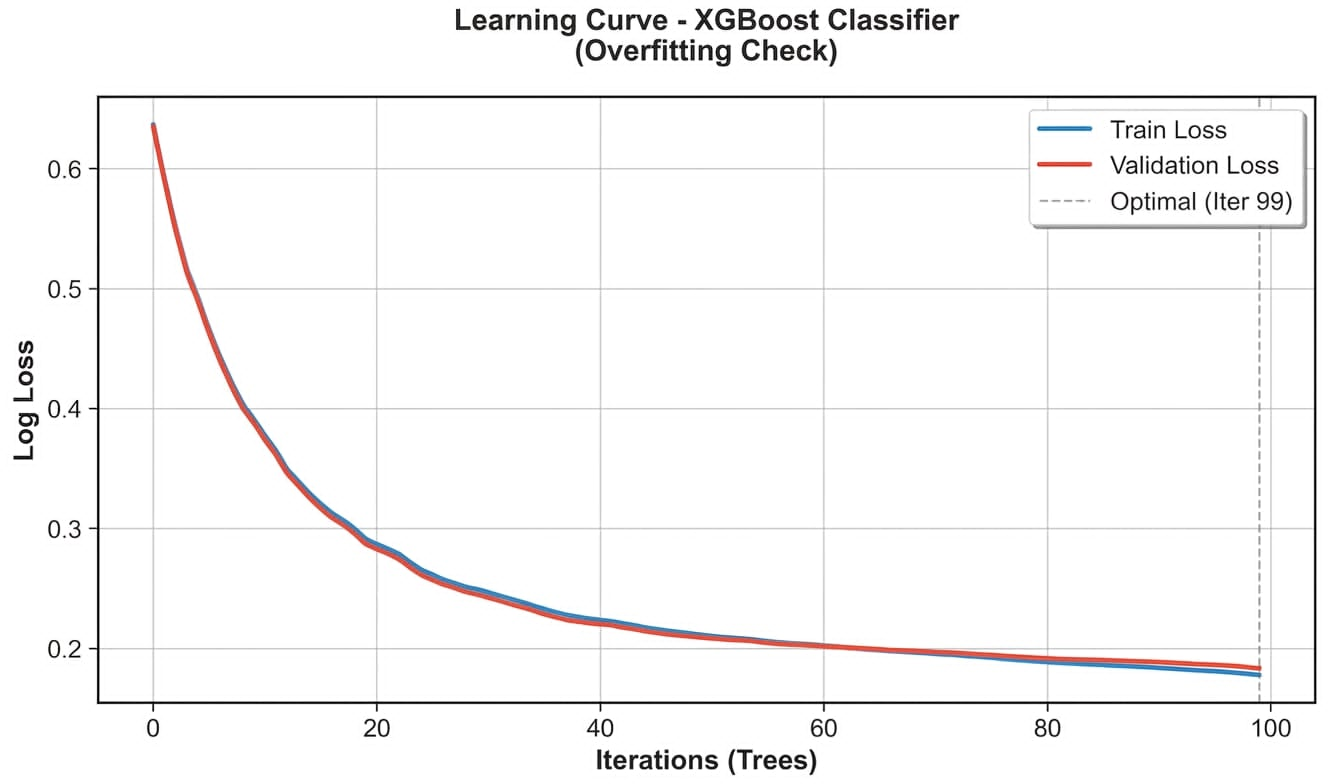
\includegraphics[width=0.92\textwidth]{figures/Overfitting Courbe.png}
\caption{XGBoost learning curve (overfitting check): train loss and validation loss
         converge smoothly over 100 boosting iterations with no divergence,
         confirming a well-controlled generalisation gap. The optimal stopping
         point is reached at iteration~99.}
\label{fig:xgboost-learning-curve}
\end{figure}
\noindent Train and validation log-loss tracks are nearly indistinguishable throughout
the 100 boosting rounds, confirming that XGBoost does not overfit on this dataset.
Extra Trees, by contrast, collapsed on the test set (F1\,$=0.53$) despite a high
training score, highlighting the danger of over-randomised ensembles on imbalanced data.

\begin{quote}
\textbf{Important note.} Near-perfect ROC-AUC ($=1.0$) warrants ongoing monitoring:
the target is derived from the rules score (Equation~\ref{eq:risk-target}), so the
model learns to \emph{replicate} the official scoring policy from antecedent
attributes. This is intentional for \textbf{screening consistency}, but SHAP and
disagreement alerts (Phase~5) remain essential to catch edge cases the rules
under-weight.
\end{quote}

\subsection{SHAP Explainability}

\subsubsection{Theoretical Foundation}

\textbf{SHAP} (SHapley Additive exPlanations) is a model-agnostic interpretability
framework introduced by Lundberg and Lee (2017) \cite{lundberg2017} that
derives from cooperative game theory. For a customer $i$ with feature vector
$\mathbf{x}_i$, the SHAP value $\phi_j(i)$ of feature $j$ is defined as the
\emph{average marginal contribution} of that feature across all possible subsets
(coalitions) of the other features:
\begin{equation}
\phi_j(i) = \sum_{S \subseteq \mathcal{F} \setminus \{j\}}
\frac{|S|!\,(|\mathcal{F}|-|S|-1)!}{|\mathcal{F}|!}
\Big[f_{S\cup\{j\}}(\mathbf{x}_{S\cup\{j\}}) - f_S(\mathbf{x}_S)\Big]
\label{eq:shap-value}
\end{equation}
where $\mathcal{F}$ is the full feature set and $f_S$ is the model's expected
prediction conditioned on the subset $S$.

For any input, the SHAP values satisfy \textbf{local accuracy}:
\begin{equation}
f(\mathbf{x}_i) = \mathbb{E}[f(\mathbf{X})] + \sum_{j=1}^{p} \phi_j(i)
\label{eq:shap-local-accuracy}
\end{equation}
meaning the model output is exactly decomposed into an additive sum of per-feature
contributions anchored at the global mean prediction.

\subsubsection{SHAP in the ATB Context}

Three regulatory and operational constraints made SHAP indispensable:

\begin{enumerate}
    \item \textbf{Regulatory explainability (KYC/AML compliance).} Tunisian banking
          regulations and BCT prudential guidelines require that risk decisions be
          justifiable to auditors. A black-box XGBoost output of ``91\% high-risk''
          is insufficient; SHAP converts it into an auditable statement: ``KYC
          incompleteness contributes $-4.8$ units, overdraft accounts $+2.1$ units.''
    \item \textbf{Model validation and trust.} For the PFE jury and for ATB risk
          managers accepting the platform, SHAP global rankings confirm that the
          model has learned \emph{business-meaningful} patterns (KYC status,
          overdraft, salary pressure) rather than spurious correlations.
    \item \textbf{Disagreement alert investigation.} When the ML model flags a
          customer as high-risk but the rules engine gives a LOW tier (the primary
          alert type), the compliance officer must decide whether to escalate.
          SHAP provides the \emph{feature-level rationale} driving the ML flag,
          enabling an informed manual review without re-running the model.
\end{enumerate}

\subsubsection{Global SHAP Analysis --- Beeswarm Plot}

Global interpretability is produced in \texttt{04\_shap\_explainability.ipynb}
using \texttt{shap.TreeExplainer} on the production XGBoost pipeline.
Figure~\ref{fig:shap-summary-atb} shows the resulting beeswarm plot
(\texttt{outputs/shap\_summary.png}): each dot represents one customer;
dot colour encodes feature value (red $=$ high, blue $=$ low); horizontal
position encodes SHAP impact on $P(\text{high risk})$.

\begin{figure}[H]
\centering
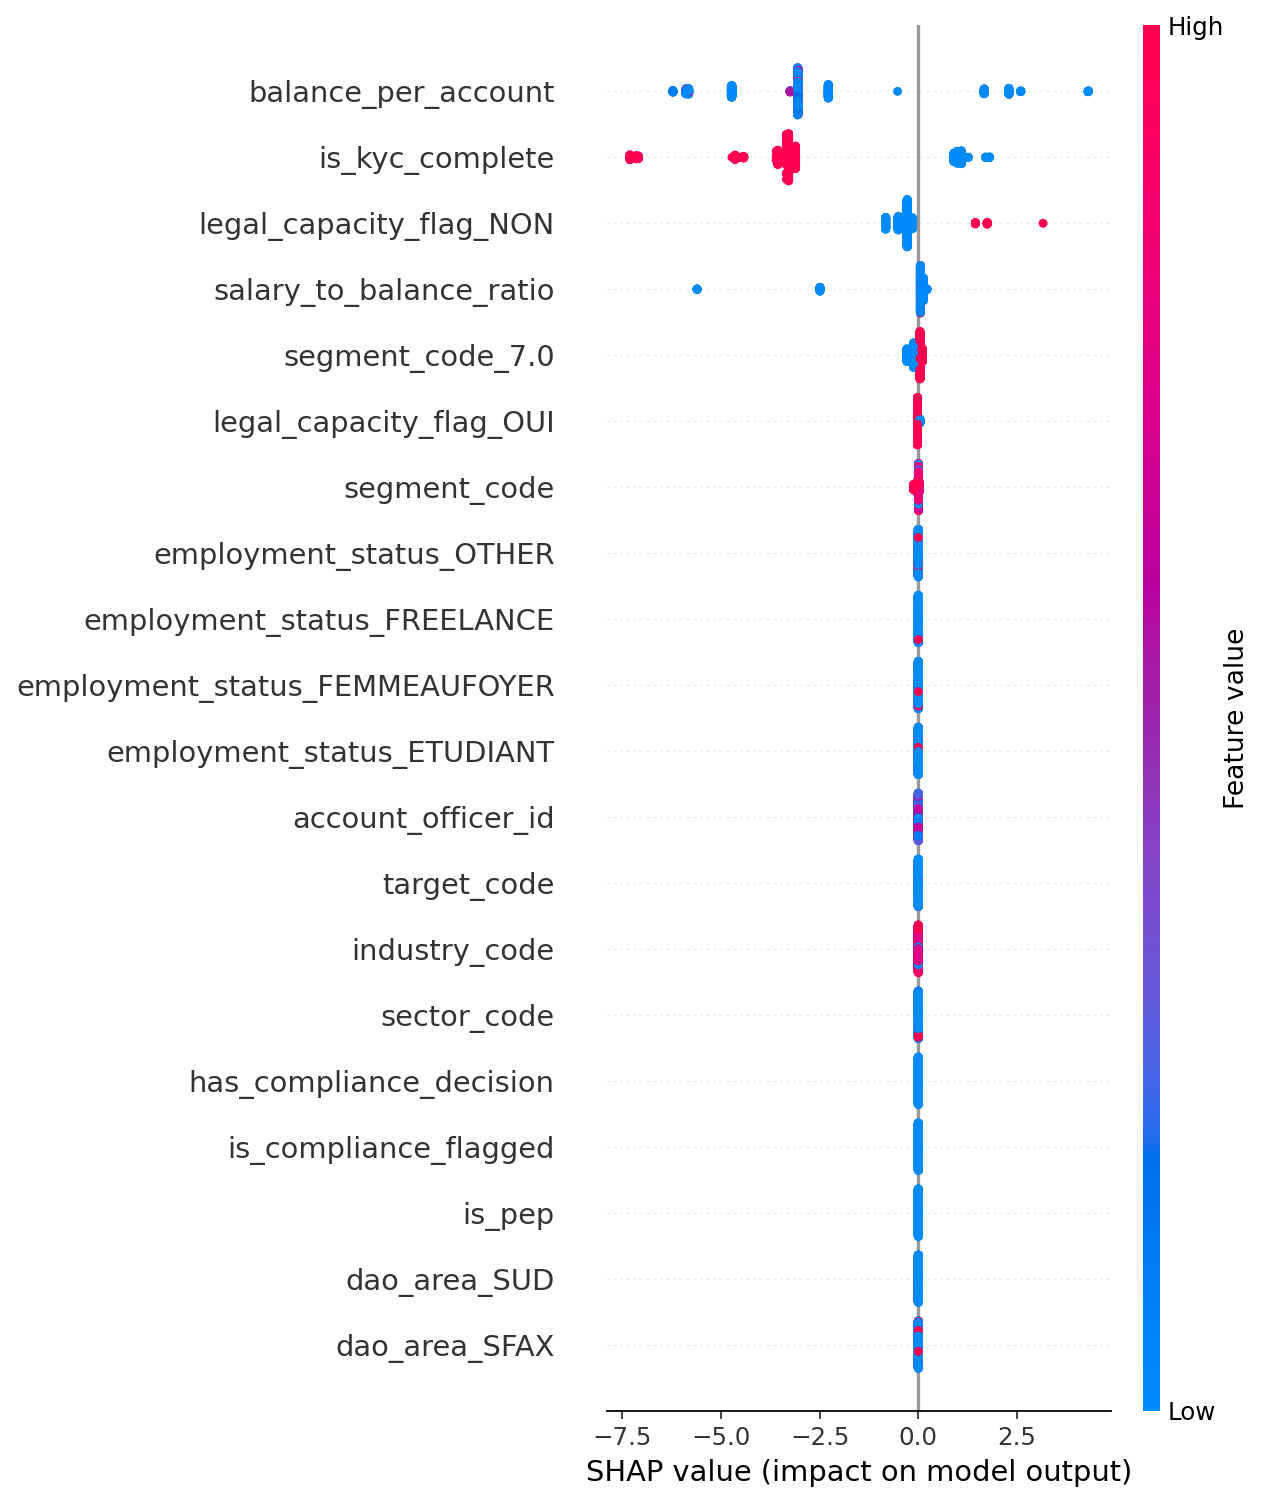
\includegraphics[width=0.90\textwidth]{figures/shap_summary.png}
\caption{Global SHAP features impact.}
\label{fig:shap-summary-atb}
\end{figure}
\noindent Each dot is one customer; colour encodes feature value
(red $=$ high); horizontal position is SHAP impact. Top drivers
(\texttt{balance\_per\_account}, \texttt{is\_kyc\_complete}, legal-capacity and
salary-to-balance ratio) align with the three-pillar rules logic.

\textbf{Key findings from Figure~\ref{fig:shap-summary-atb}:}
\begin{itemize}
    \item \textbf{\texttt{balance\_per\_account}} is the single strongest driver:
          customers with a high balance per account (red dots) shift
          $P(\text{high risk})$ \emph{upward} by up to $+3.5$ SHAP units, reflecting
          that concentrated portfolios with few accounts are atypical and flagged.
    \item \textbf{\texttt{is\_kyc\_complete}} produces the sharpest binary separation:
          KYC-complete customers (red) accumulate strong negative SHAP values
          (push toward low risk), while incomplete KYC (blue) pushes strongly
          toward high risk directly echoing the compliance pillar of the rules
          engine.
    \item \textbf{\texttt{legal\_capacity\_flag\_NON}} and \textbf{\texttt{salary\_to\_balance\_ratio}}
          are the third and fourth drivers, confirming that legal restrictions and
          income-to-liquidity pressure are critical antecedents the tree model has
          discovered independently from the three-pillar formula.
    \item Segmentation variables (\texttt{segment\_code}, \texttt{employment\_status})
          appear in the lower tier, providing supplementary context but not decisive
          powerconsistent with the business expectation that KYC and financial
          behaviour dominate.
\end{itemize}

\textbf{SHAP and the Dual-Layer Coherence Test.} The top SHAP drivers align with
the three pillars of the rules engine (compliance index $\leftrightarrow$
\texttt{is\_kyc\_complete}, \texttt{is\_pep}; financial fragility $\leftrightarrow$
\texttt{balance\_per\_account}, \texttt{salary\_to\_balance\_ratio}). This structural
alignment validates that the XGBoost model has learned the \emph{same risk logic}
as the deterministic rules but from raw attributes providing an independent
cross-check of the scoring methodology.

%======================================================================
\section{Model Deployment}
\label{sec:phase5_streamlit}
%======================================================================

\subsection{Integration Overview}

The ML module is integrated into the existing role-based Streamlit dashboard
without modifying any of the Release~2 navigation or access-control structure.
Three new pages are added:

\begin{table}[H]
\centering
\caption{New ML pages integrated into the Streamlit dashboard}
\label{tab:streamlit-ml-pages}
\begin{tabular}{|p{4.5cm}|p{9cm}|}
\hline
\textbf{Page} & \textbf{Purpose} \\
\hline
ML Risk Intelligence & Operational scoring hub: live lookup, batch scoring, evaluation curves, model metrics, and the full predictor form \\
MLflow Model Registry & Governance view: production model card, registered versions, and recent training run history \\
ML \& Risk Scoring Guide & Reference aide for the PFE defence: explains the rules-vs-ML architecture, metric definitions, and KYC flag mapping \\
\hline
\end{tabular}
\end{table}

The \textbf{ML Risk Intelligence} page exposes five tabs, each mapping to a
Sprint~4 user story:

\begin{table}[H]
\centering
\caption{ML Risk Intelligence tabs functionality}
\label{tab:ml-tabs}
\begin{tabular}{|l|l|p{7cm}|}
\hline
\textbf{Tab} & \textbf{US} & \textbf{Description} \\
\hline
Live demo & US~11 & Lookup \texttt{customer\_id}, side-by-side rules vs ML \\
Batch \& alerts & US~11, US~14 & Score 500--8\,000 customers; disagreement CSV export \\
Curves \& SHAP & US~12 & ROC/PR, confusion matrix, SHAP image, threshold what-if \\
XGBoost metrics & US~10 & KPI row + bar charts vs Random Forest \\
Full predictor & US~11 & Manual 25+ field form for what-if profiling \\
\hline
\end{tabular}
\end{table}

%----------------------------------------------------------------------
\subsection{Live Demo}
%----------------------------------------------------------------------

The live demo allows a compliance officer to look up any customer by identifier
and receive a side-by-side comparison of the two risk layers:

\begin{itemize}
    \item \textbf{Rules engine}: the official deterministic score, risk tier, and HIGH/LOW classification.
    \item \textbf{Machine learning}: the XGBoost probability score with an adjustable threshold slider.
    \item \textbf{Agreement status}: a clear visual indicator --- either MATCH or REVIEW --- flagging cases where the two layers disagree.
\end{itemize}

A pillar breakdown (compliance index, overdraft count, KYC flags) is also
displayed to support the officer's manual investigation.

% --- SCREENSHOT: Streamlit Live demo tab (customer ID lookup, side-by-side cards)
\begin{figure}[H]
\centering
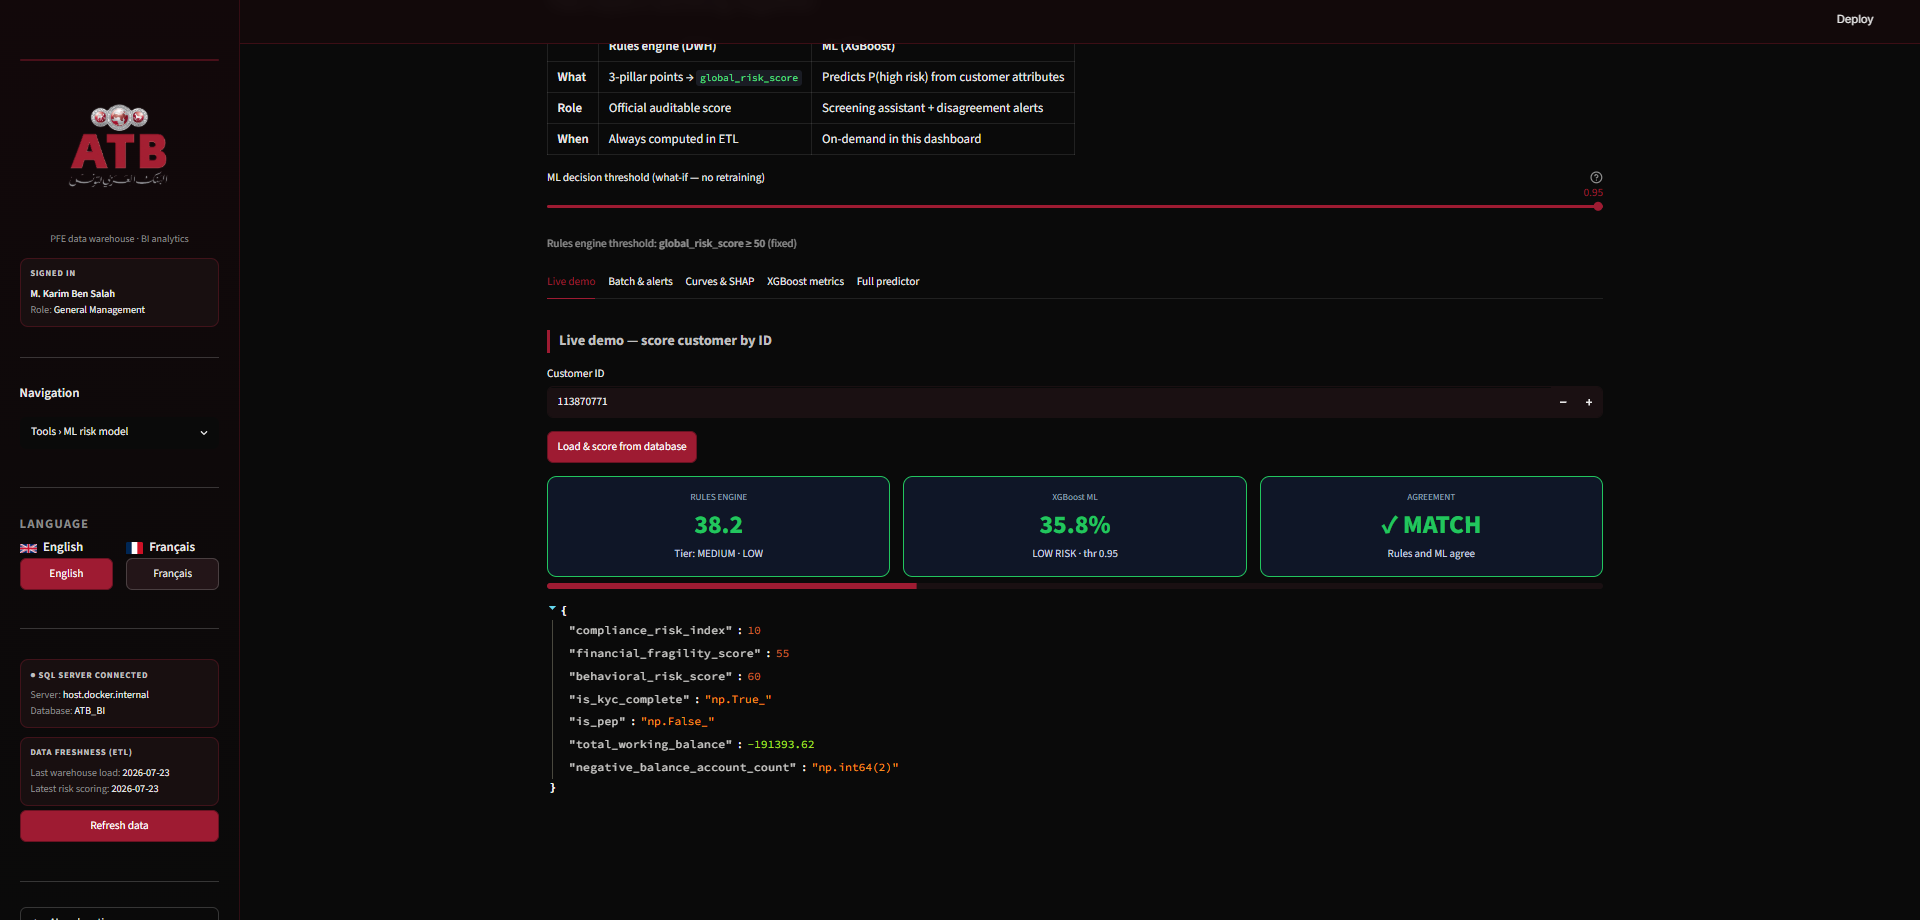
\includegraphics[width=0.95\textwidth]{figures/ml_live_demo.png}
\caption{Streamlit \emph{Live demo} showing single result for customer}
\label{fig:ml-live-demo}
\end{figure}
\noindent Side-by-side cards show the official GRS/tier next to
the ML probability and MATCH/REVIEW status, with pillar breakdowns for manual
investigation.

%----------------------------------------------------------------------
\subsection{Batch Scoring and Disagreement Alerts}
%----------------------------------------------------------------------

Batch mode scores a configurable population of customers and computes three
key indicators:
\begin{itemize}
    \item \textbf{Agreement rate} between the rules tier and the ML label.
    \item \textbf{ML high / Rules low} cases --- the primary alert population
          (customers the model considers high-risk that the rules engine has
          not yet escalated).
    \item \textbf{Rules high / ML low} cases --- a secondary review population.
\end{itemize}

The visual analytics panel includes the ML probability distribution histogram
and a scatter plot of the rules score against the ML probability --- allowing
a risk manager to immediately see where the two layers diverge. Disagreement
alerts can be downloaded as a CSV file for offline review.

% --- SCREENSHOT: Streamlit Batch & alerts tab (KPIs + alert table)
\begin{figure}[H]
\centering
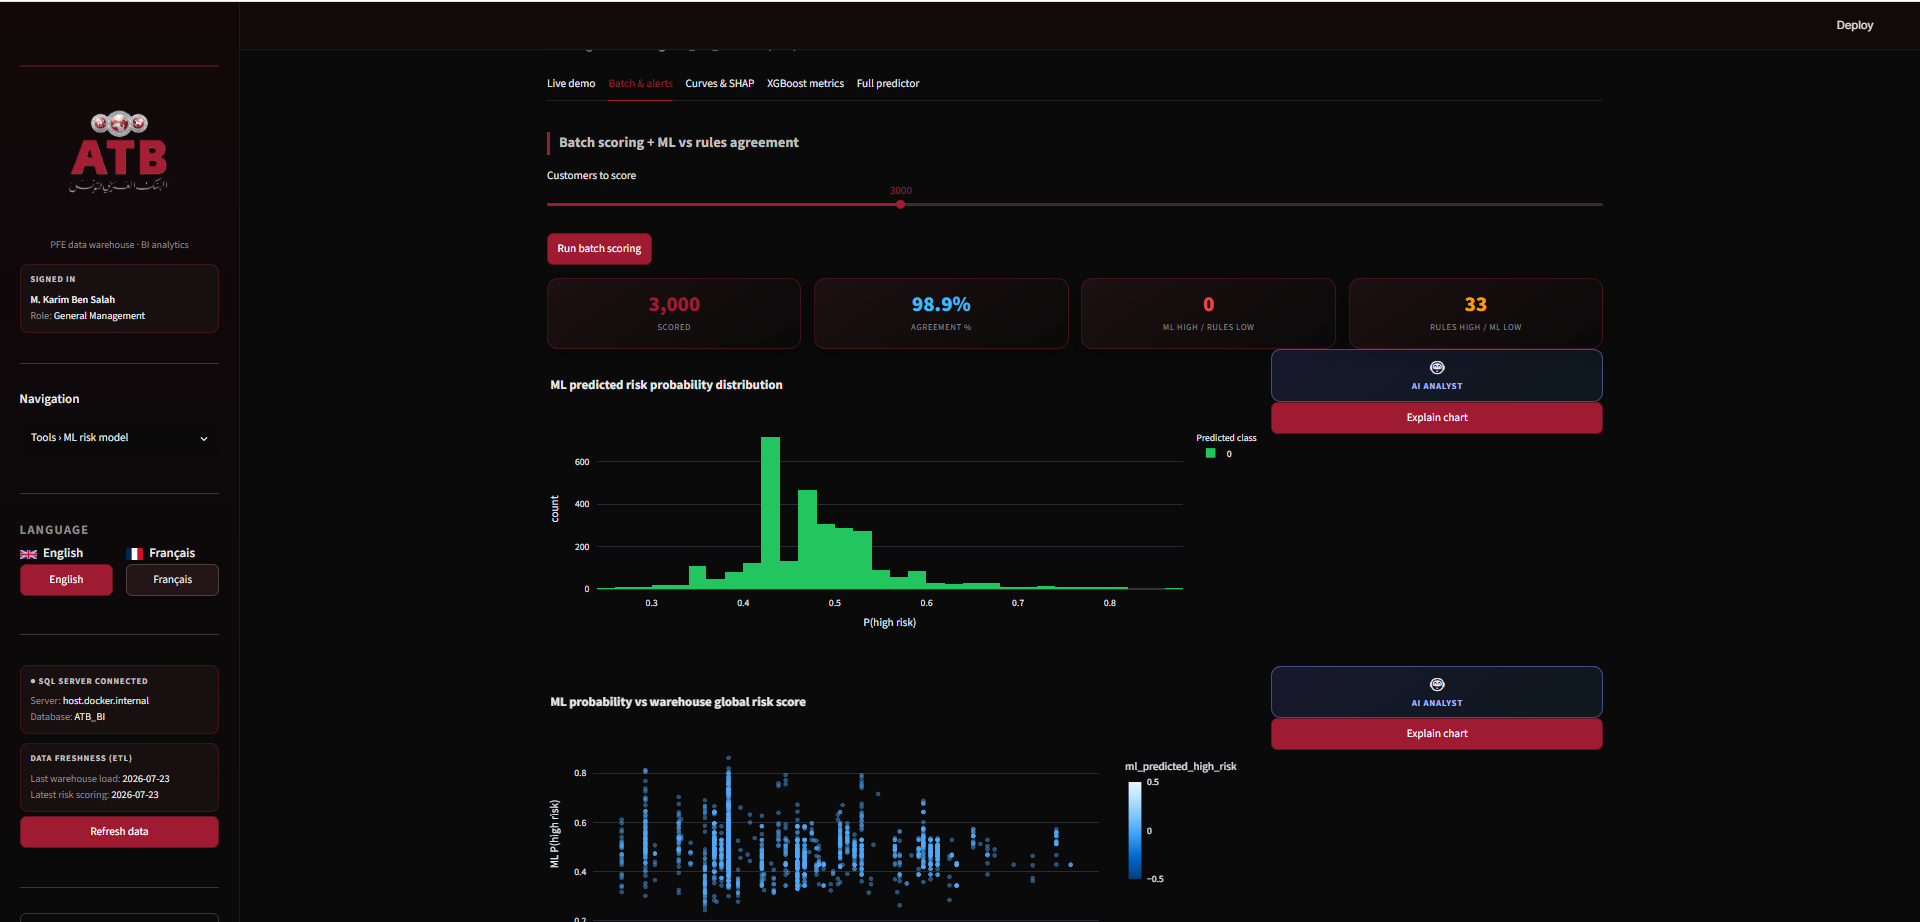
\includegraphics[width=0.95\textwidth]{figures/ml_batch_alerts.png}
\caption{Streamlit --- \emph{Batch \& alerts} tab: agreement KPIs and disagreement alert list}
\label{fig:ml-batch-alerts}
\end{figure}
\noindent Population scoring reports agreement rate plus the two
disagreement directions; the CSV export feeds the compliance alert inbox without
re-running inference.

%----------------------------------------------------------------------
\subsection{Evaluation Curves and SHAP}
%----------------------------------------------------------------------

This tab provides a unified model quality view:
\begin{enumerate}
    \item Dual-panel \textbf{ROC and Precision--Recall curves} with AUC annotations.
    \item A \textbf{confusion matrix} heatmap updated dynamically as the threshold slider is moved.
    \item The embedded \textbf{SHAP global importance} beeswarm plot.
    \item A \textbf{threshold sensitivity} chart showing how precision, recall,
          and F1 trade off across the full $[0, 1]$ range.
\end{enumerate}

The Gemini AI explainer is available on this tab, allowing a compliance
officer to request a plain-language interpretation of the probability
distribution without needing any statistical background.

%----------------------------------------------------------------------
\subsection{Model Metrics}
%----------------------------------------------------------------------

The metrics tab surfaces the production model card: algorithm name, ROC-AUC, F1,
precision, recall, and PR-AUC. Bar charts compare XGBoost against Random Forest
across each metric, and a gallery of training output charts is displayed for
training transparency.

\begin{figure}[H]
\centering
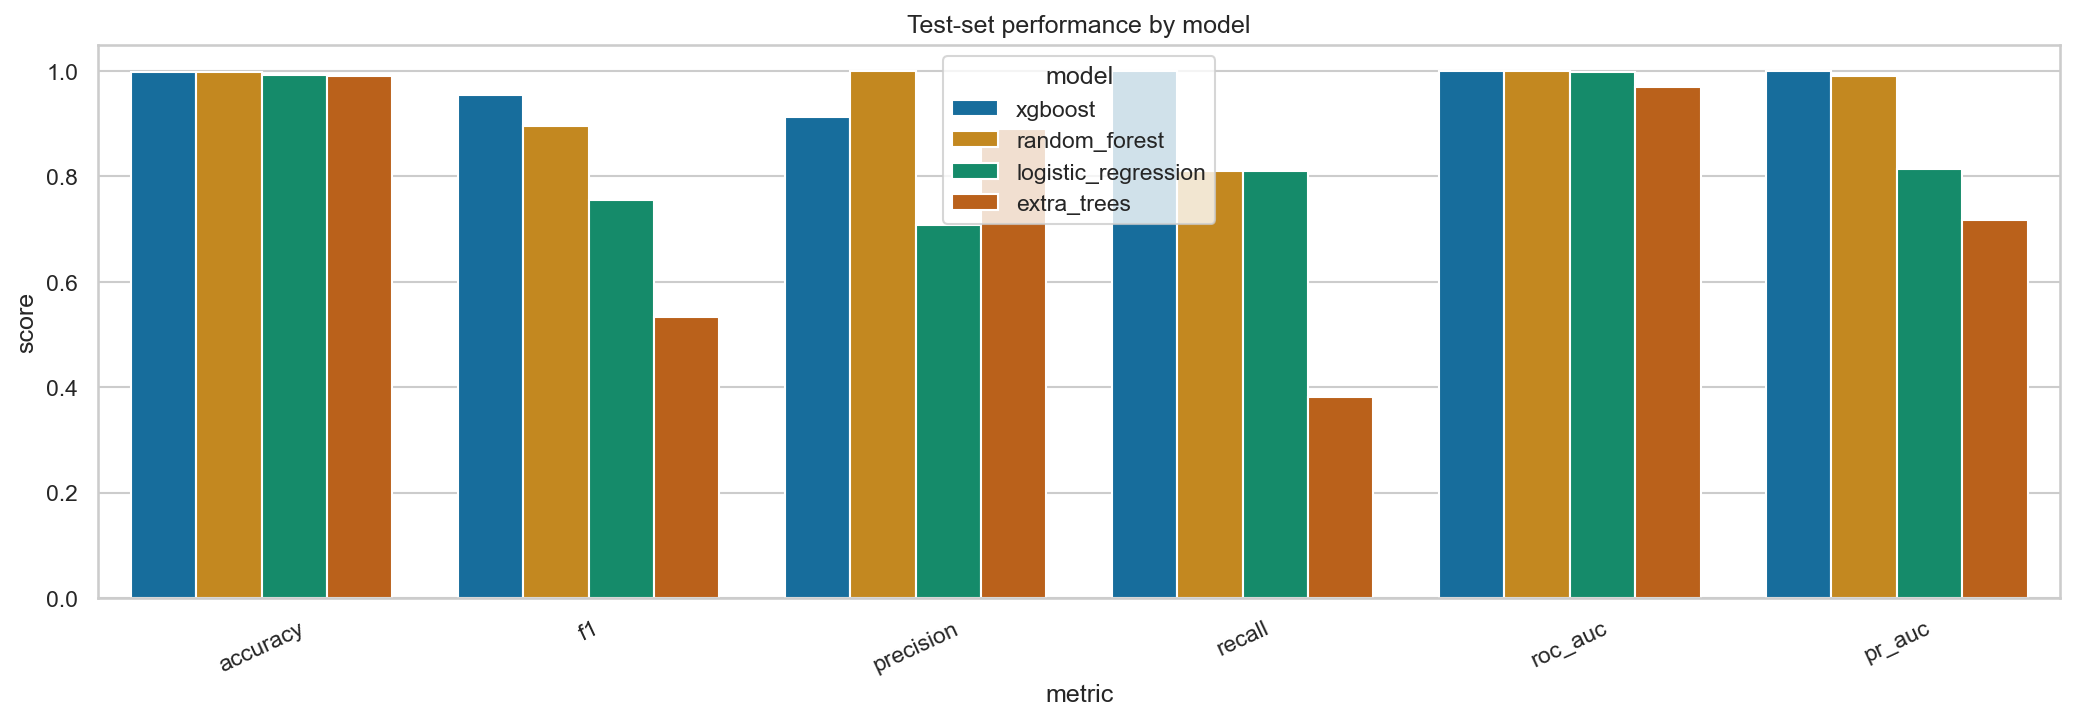
\includegraphics[width=0.92\textwidth]{figures/05_test_metrics_comparison.png}
\caption{Model metrics comparison --- test performance across key classification metrics}
\label{fig:ml-metrics-tab}
\end{figure}
\noindent The same numbers as Table~\ref{tab:all-models-comparison}
are exposed to non-technical users as KPI cards and bars inside Streamlit.

%----------------------------------------------------------------------
\subsection{Tab 5 --- Full Predictor}
%----------------------------------------------------------------------

The \textbf{Full predictor} tab is the most comprehensive interactive tool in
the ML Risk Intelligence module. It exposes \emph{all} 25+ training-time
attributes in a structured three-section form, allowing a risk analyst to
construct a hypothetical customer profile from scratch and obtain an
immediate XGBoost prediction \emph{without} any database connection.

The form is organised into three blocks that mirror the model's feature namespaces:
\begin{enumerate}
    \item \textbf{Customer profile}: gender, marital status, employment status,
          residence status, customer tenure (days), days since last KYC review,
          monthly salary (DT), number of dependants, and segment code.
    \item \textbf{Accounts \& balances}: number of bank accounts, average and total
          working balances (DT), and number of overdraft accounts.
    \item \textbf{Segmentation \& compliance}: sector code, DAO branch area,
          industry code, target segment code, KYC completeness flag, PEP
          (Politically Exposed Person) flag, compliance-flagged status,
          has-compliance-decision flag, client nature, legal capacity, and
          beneficial owner indicator.
\end{enumerate}

On submit, \texttt{ml\_service.predict\_single()} applies the production
\texttt{ColumnTransformer} (imputation $\rightarrow$ one-hot encoding) and
XGBoost pipeline to the manual form values and returns:
\begin{itemize}
    \item $P(\text{high risk})$ as a percentage gauge.
    \item Binary label (\textbf{HIGH RISK} / \textbf{LOW RISK}) at the
          production threshold $\approx 0.953$.
    \item Confidence percentage and threshold reminder.
\end{itemize}

\begin{figure}[H]
\centering
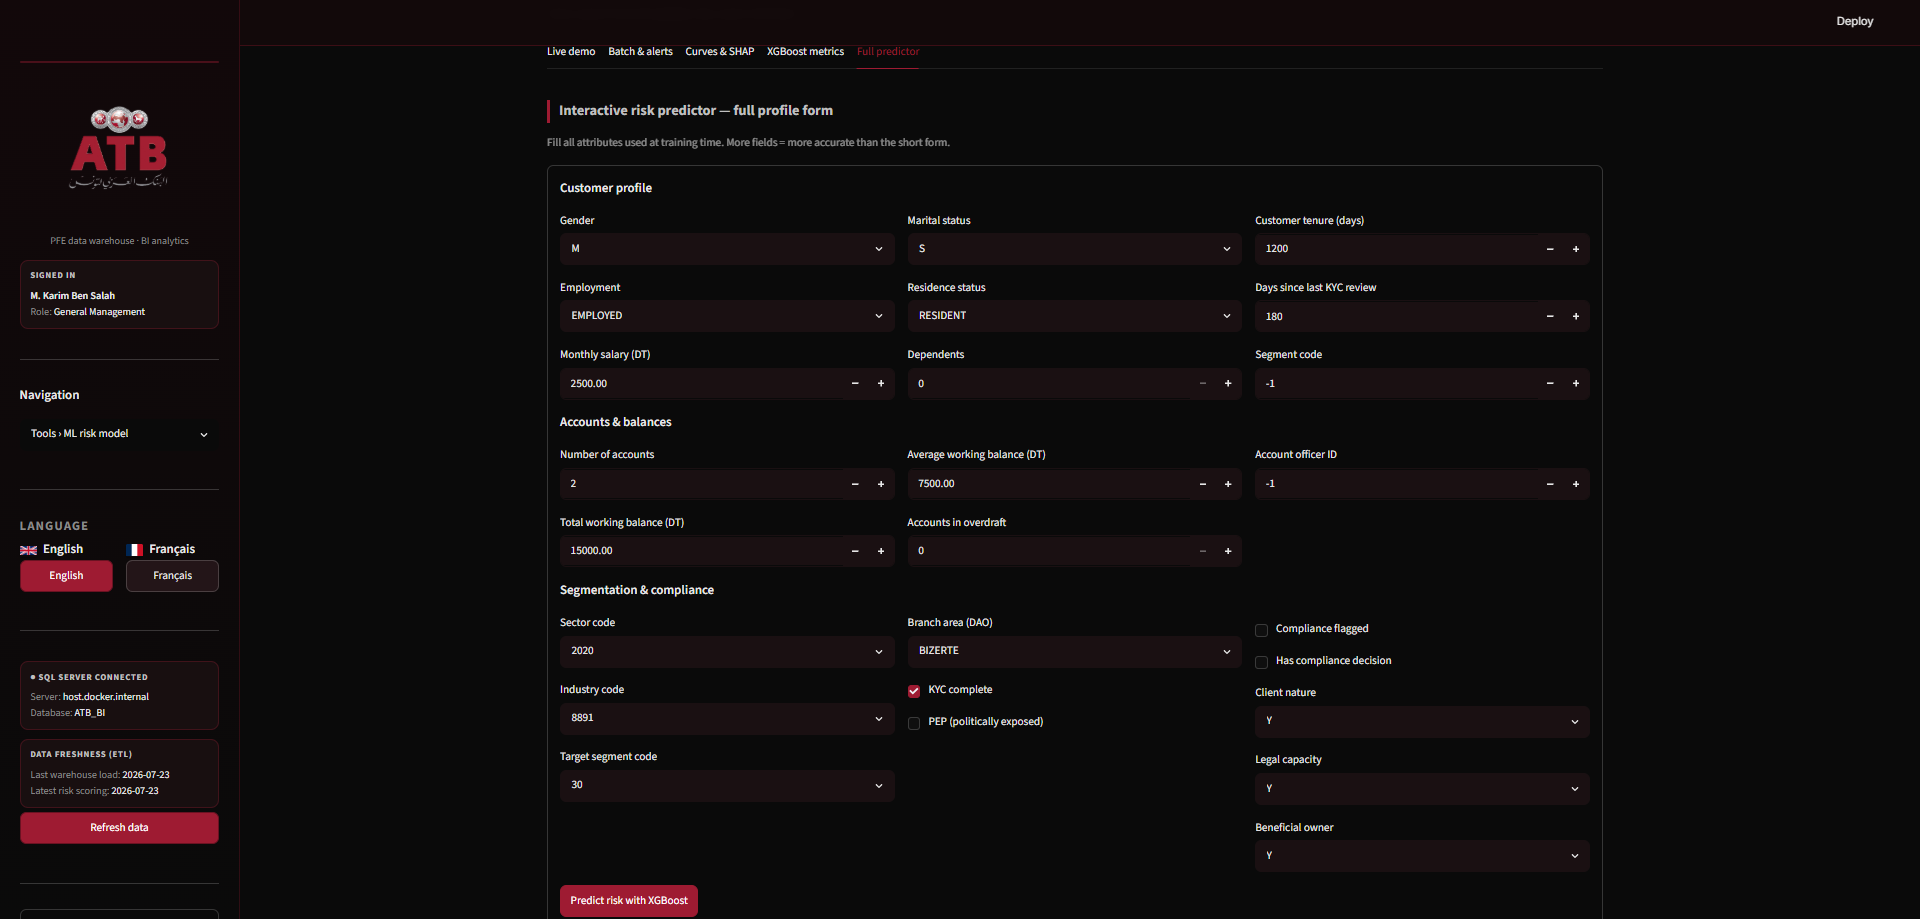
\includegraphics[width=0.95\textwidth]{figures/FullpRedictor.png}
\caption{Full predictor --- interactive what-if form over 25+ training attributes}
\label{fig:full-predictor}
\end{figure}
\noindent Analysts build a hypothetical profile (demographics,
balances, KYC/PEP flags) and obtain $P(\text{high risk})$ instantly --- useful
for workshops such as ``what if KYC becomes incomplete?''.

This tool is particularly valuable for \textbf{what-if workshops}:
\begin{itemize}
    \item ``What happens to risk probability if KYC becomes incomplete
          (\texttt{is\_kyc\_complete} = 0)?'' $\rightarrow$ typically a sharp rise
          driven by the SHAP dominance of \texttt{is\_kyc\_complete}.
    \item ``If overdraft accounts increase from 0 to 2, does the customer cross
          the HIGH threshold?'' $\rightarrow$ the form recalculates in real time.
    \item ``Is a new freelancer (tenure $<$ 365 days, PEP = true) high risk
          even with a positive salary?'' $\rightarrow$ actionable before
          account opening.
\end{itemize}

%======================================================================
\section{Monitoring \& Maintenance}
\label{sec:phase6_monitoring}
%======================================================================

\subsection{MLflow Model Registry Governance}

The \textbf{MLflow Model Registry} page in the dashboard provides governance
visibility for auditors and the project jury:
\begin{itemize}
    \item \textbf{Production model card}: name, version, stage, algorithm, and all key metrics.
    \item \textbf{Version history}: a table of all registered model versions with their lifecycle stage.
    \item \textbf{Recent training run log}: recent experiment runs with ROC-AUC, F1, precision, and recall.
    \item \textbf{Batch scoring summary}: number of customers scored, ML high-risk count, and disagreement count.
\end{itemize}

\begin{figure}[H]
\centering
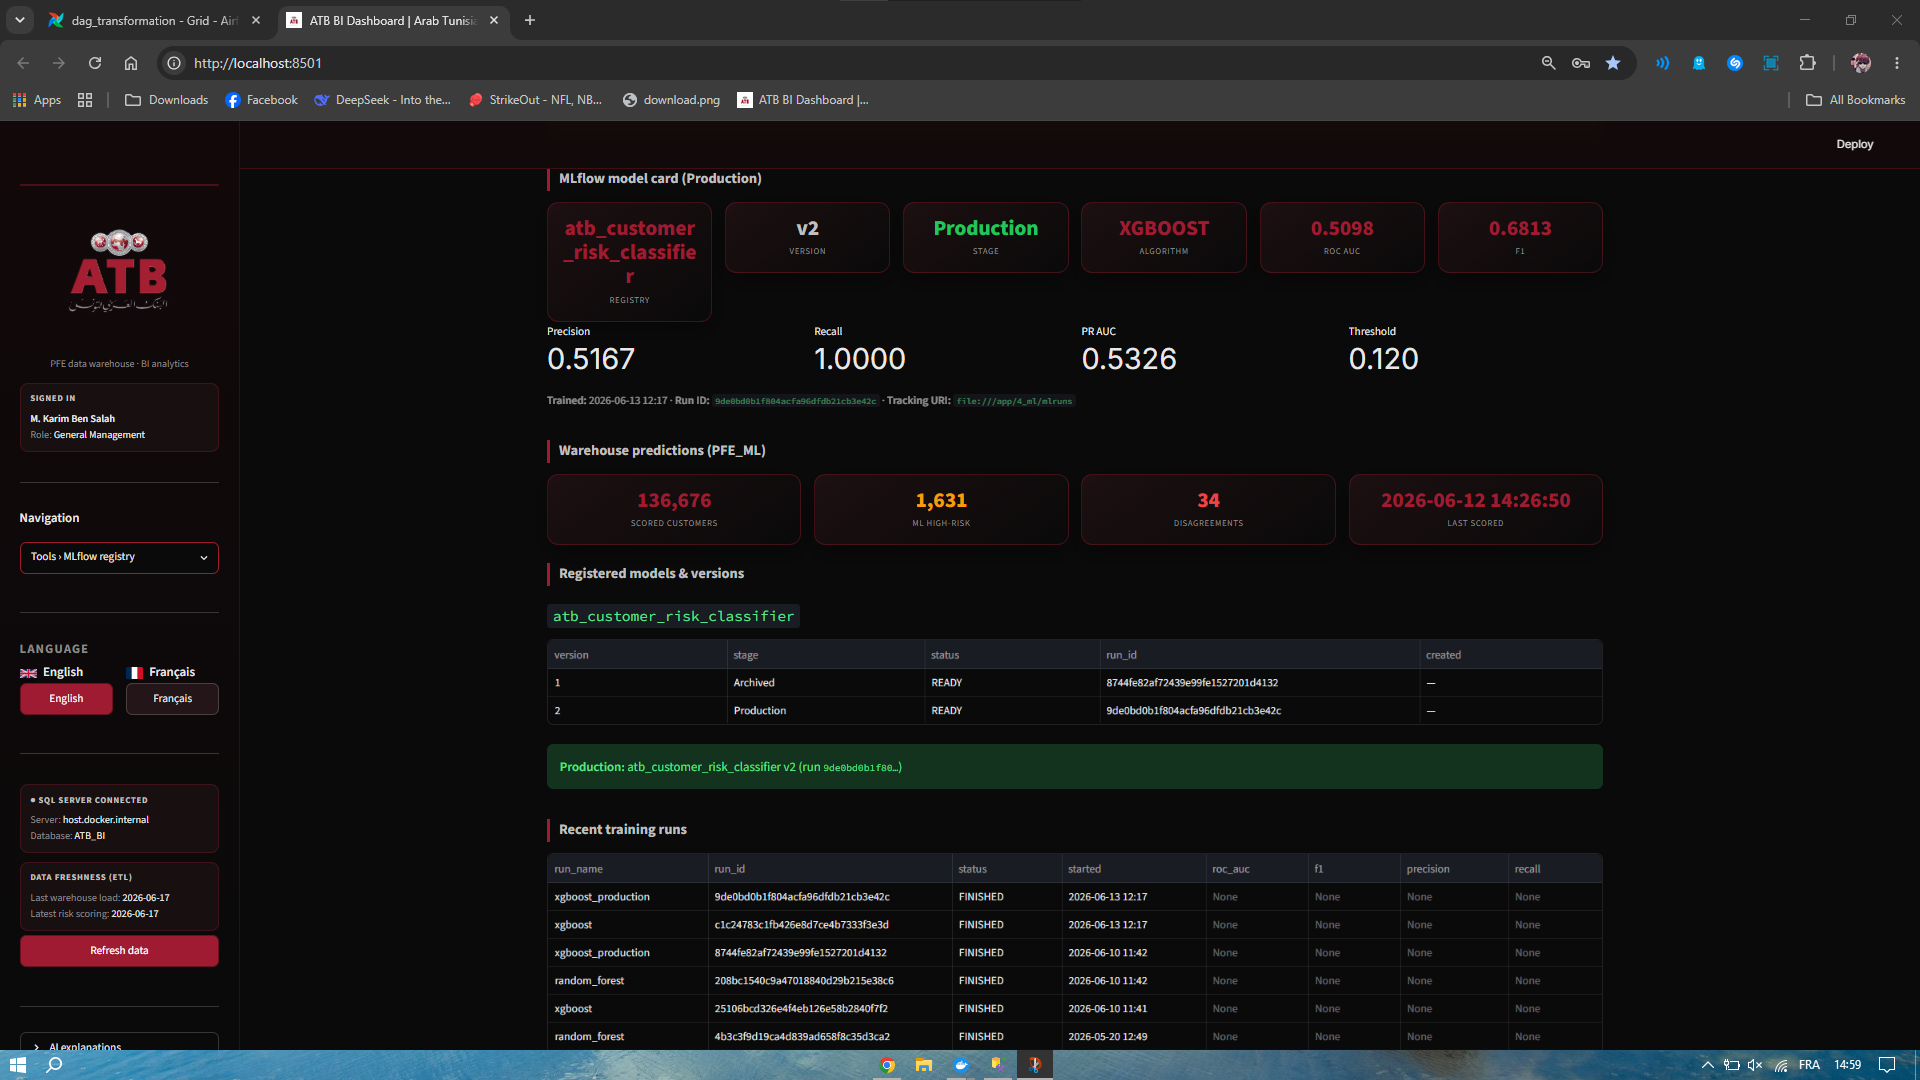
\includegraphics[width=0.95\textwidth]{figures/mlflow_registry_page.png}
\caption{MLflow Model Registry page in the dashboard}
\label{fig:mlflow-registry}
\end{figure}
\noindent Auditors and the jury see the production model card,
version history and recent runs without opening the native MLflow UI.

\subsection{Containerised Deployment and DevOps Engineering}
\label{sec:containerised_devops}

Beyond leveraging standard container images for Airbyte and Airflow, a major technical contribution of this project lies in the \textbf{custom DevOps engineering} developed to containerise the Streamlit decision application and the Machine Learning execution layer.

Rather than relying on generic off-the-shelf images, we designed and authored custom multi-stage \texttt{Dockerfile} descriptors and modular \texttt{docker-compose.yml} service specifications. This guarantees reproducible, production-grade deployment across any operating system (Windows Server, Linux, macOS) while isolating database drivers, ML models, and presentation logic.

\subsubsection{1. Custom Streamlit \& ML Container Image (\texttt{Dockerfile})}
The presentation layer and predictive model runtime are packaged into a custom Docker image (\texttt{atb-streamlit:latest}) engineered specifically for ATB's enterprise architecture. Key engineering highlights of this container include:

\begin{itemize}
    \item \textbf{Enterprise Database Connectivity:} Automatic installation and configuration of Microsoft GPG keys and native Linux ODBC drivers (\texttt{msodbcsql17} and \texttt{msodbcsql18}) required for high-throughput SQL Server connections.
    \item \textbf{Container-in-Container (DinC) Operations:} Integration of the Docker CE CLI engine within the image, allowing the dashboard to monitor and trigger container health status directly.
    \item \textbf{Bundled ML Artefacts and Codebase:} Encapsulation of the \texttt{4\_ml} serialised model pipeline, MLflow tracking stores, and Streamlit presentation codebase into a unified, version-controlled image workspace.
\end{itemize}

% --- SCREENSHOT: Add screenshot of the custom 5_reporting/streamlit/Dockerfile here
\begin{figure}[H]
\centering
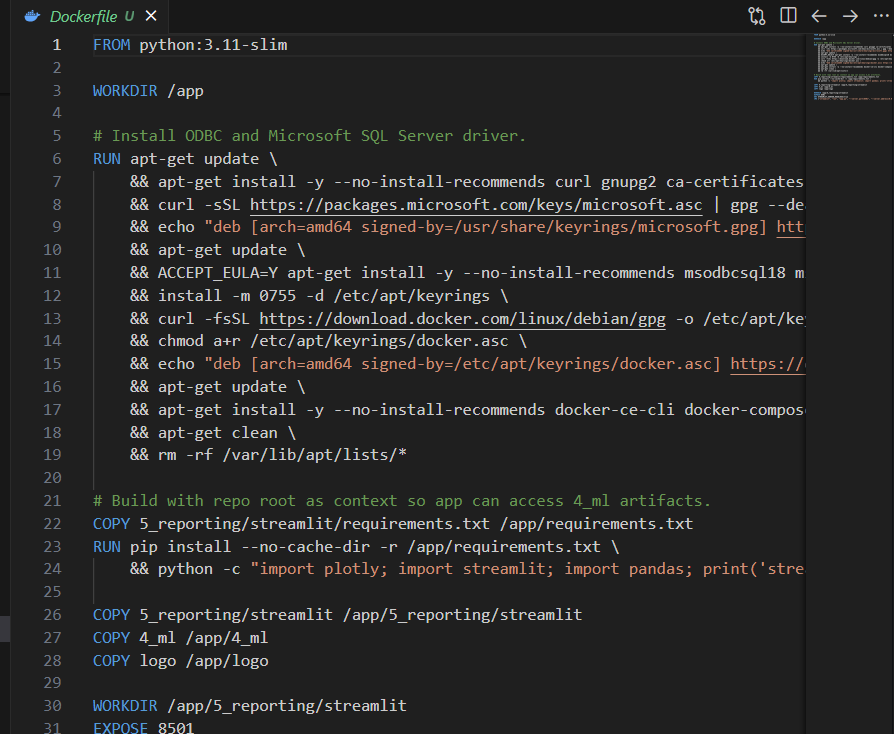
\includegraphics[width=0.88\textwidth]{figures/streamlit_dockerfile_yaml.png}
\caption{Custom Dockerfile configuration for the ATB Streamlit \& ML container}
\label{fig:streamlit-dockerfile-code}
\end{figure}
\noindent Custom Dockerfile specification for the Streamlit dashboard and ML prediction environment.

\subsubsection{2. Custom Service Orchestration}
To orchestrate the Streamlit dashboard alongside SQL Server, Airflow, and MLflow, a custom \texttt{docker-compose.yml} specification was created. This configuration defines:

\begin{itemize}
    \item \textbf{Host-Gateway Network Bridging:} Explicit mapping of \texttt{host.docker.internal:host-gateway} enabling seamless TCP communication between containerised services and the host-bound SQL Server Data Warehouse.
    \item \textbf{Volume Mounts for ML Persistence:} Volume bindings mapping Machine learning and Streamlit interface to ensure continuous persistence of MLflow experiment runs and dynamic dashboard assets.
    \item \textbf{Environment Variable Isolation:} Integration of isolated \texttt{.env} configuration files for database credentials, schema names, and MLflow tracking URIs.
\end{itemize}

% --- SCREENSHOT: Add screenshot of the custom 5_reporting/streamlit/docker-compose.yml file here
\begin{figure}[H]
\centering
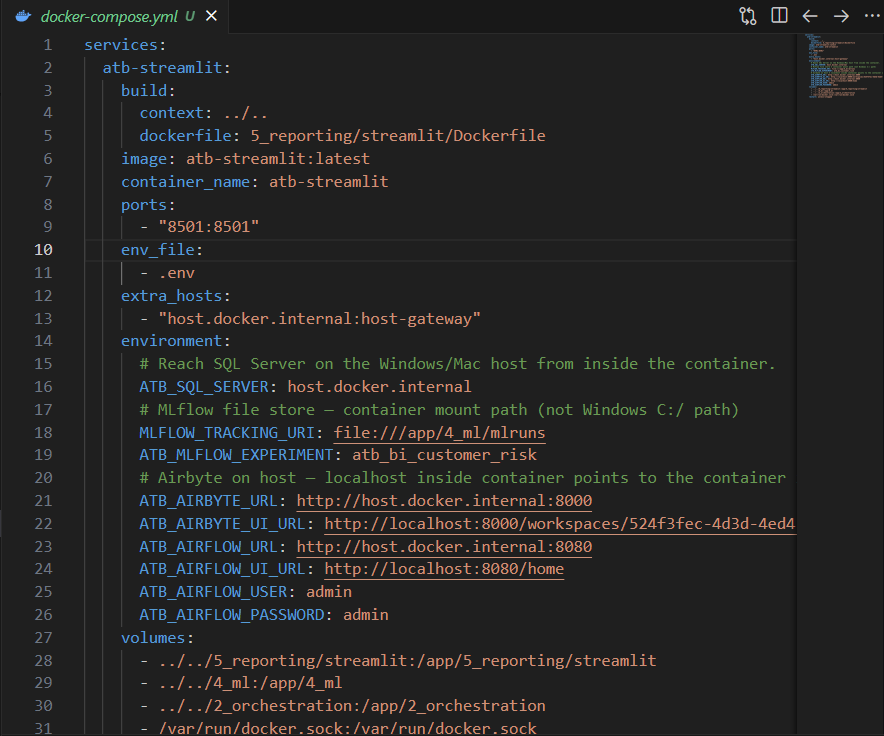
\includegraphics[width=0.88\textwidth]{figures/streamlit_docker_compose_yaml.png}
\caption{Custom docker-compose.yml orchestration file for Streamlit and ML services}
\label{fig:streamlit-docker-compose-yaml}
\end{figure}
\noindent % [USER INSTRUCTION]: Place your screenshot of 5_reporting/streamlit/docker-compose.yml above (uncomment \includegraphics).

% --- SCREENSHOT: docker ps or Docker Desktop showing atb-streamlit and container stack running
\begin{figure}[H]
\centering
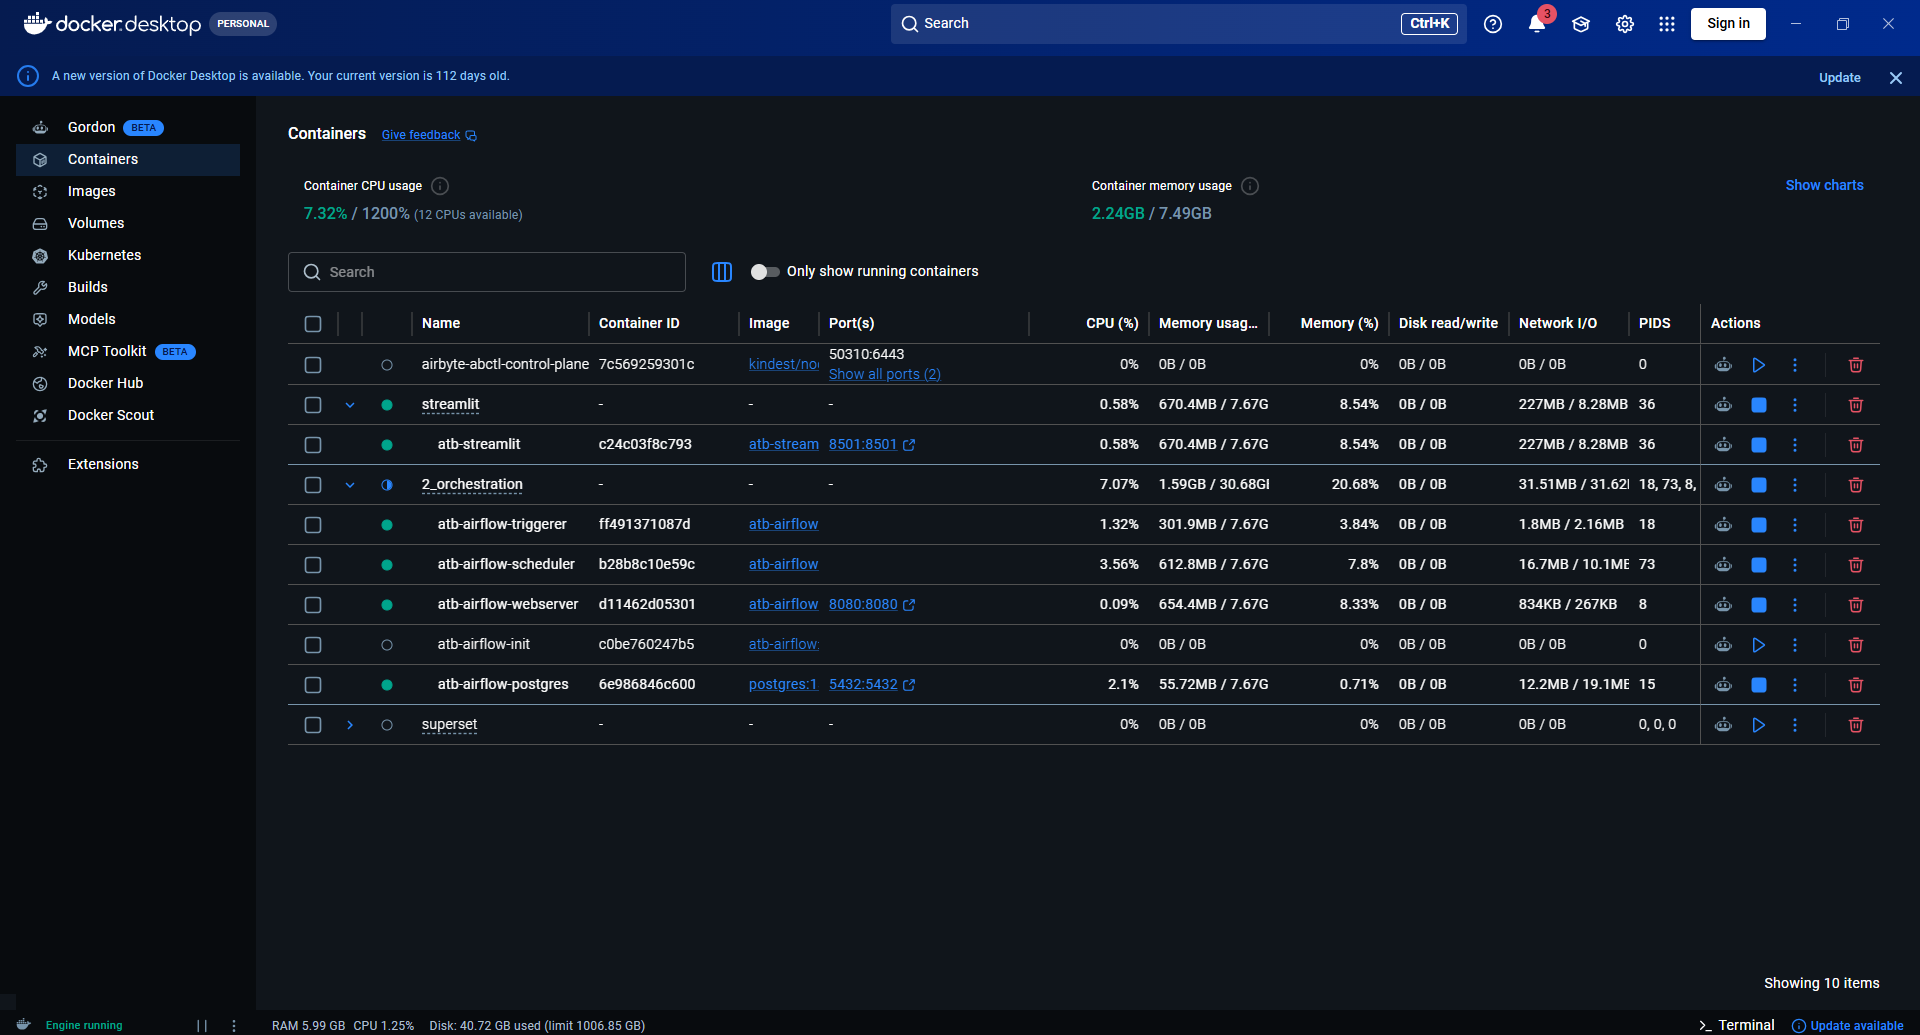
\includegraphics[width=0.85\textwidth]{figures/streamlit_docker_running.png}
\caption{Docker Desktop operational view of running containerised stack}
\label{fig:streamlit-docker}
\end{figure}
\noindent The custom dashboard image bundles ODBC drivers, Streamlit scripts, and ML artefacts, ensuring seamless, one-command deployment (\texttt{docker-compose up}) across environments.

\subsection{Automated ML Retraining with Airflow}

The orchestration layer introduced in Release~1 is extended in Sprint~4 with
a dedicated ML pipeline. Two scheduled or manually triggered workflows handle
the full training-to-scoring lifecycle:

\begin{table}[H]
\centering
\caption{Airflow DAGs for ML orchestration}
\label{tab:airflow-ml-dags}
\begin{tabular}{|p{4cm}|l|p{6.5cm}|}
\hline
\textbf{DAG} & \textbf{Schedule} & \textbf{Tasks} \\
\hline
ML Pipeline & Manual / triggered & Train model $\rightarrow$ validate artefact $\rightarrow$ write predictions \\
Master Pipeline & Daily 02:00 UTC & Ingestion $\rightarrow$ transformation $\rightarrow$ quality $\rightarrow$ ML (Sundays) \\
\hline
\end{tabular}
\end{table}

The master pipeline includes a short-circuit condition so that ML retraining
only executes on Sundays, or when manually forced, preventing unnecessary
daily computation costs.

\begin{figure}[H]
\centering
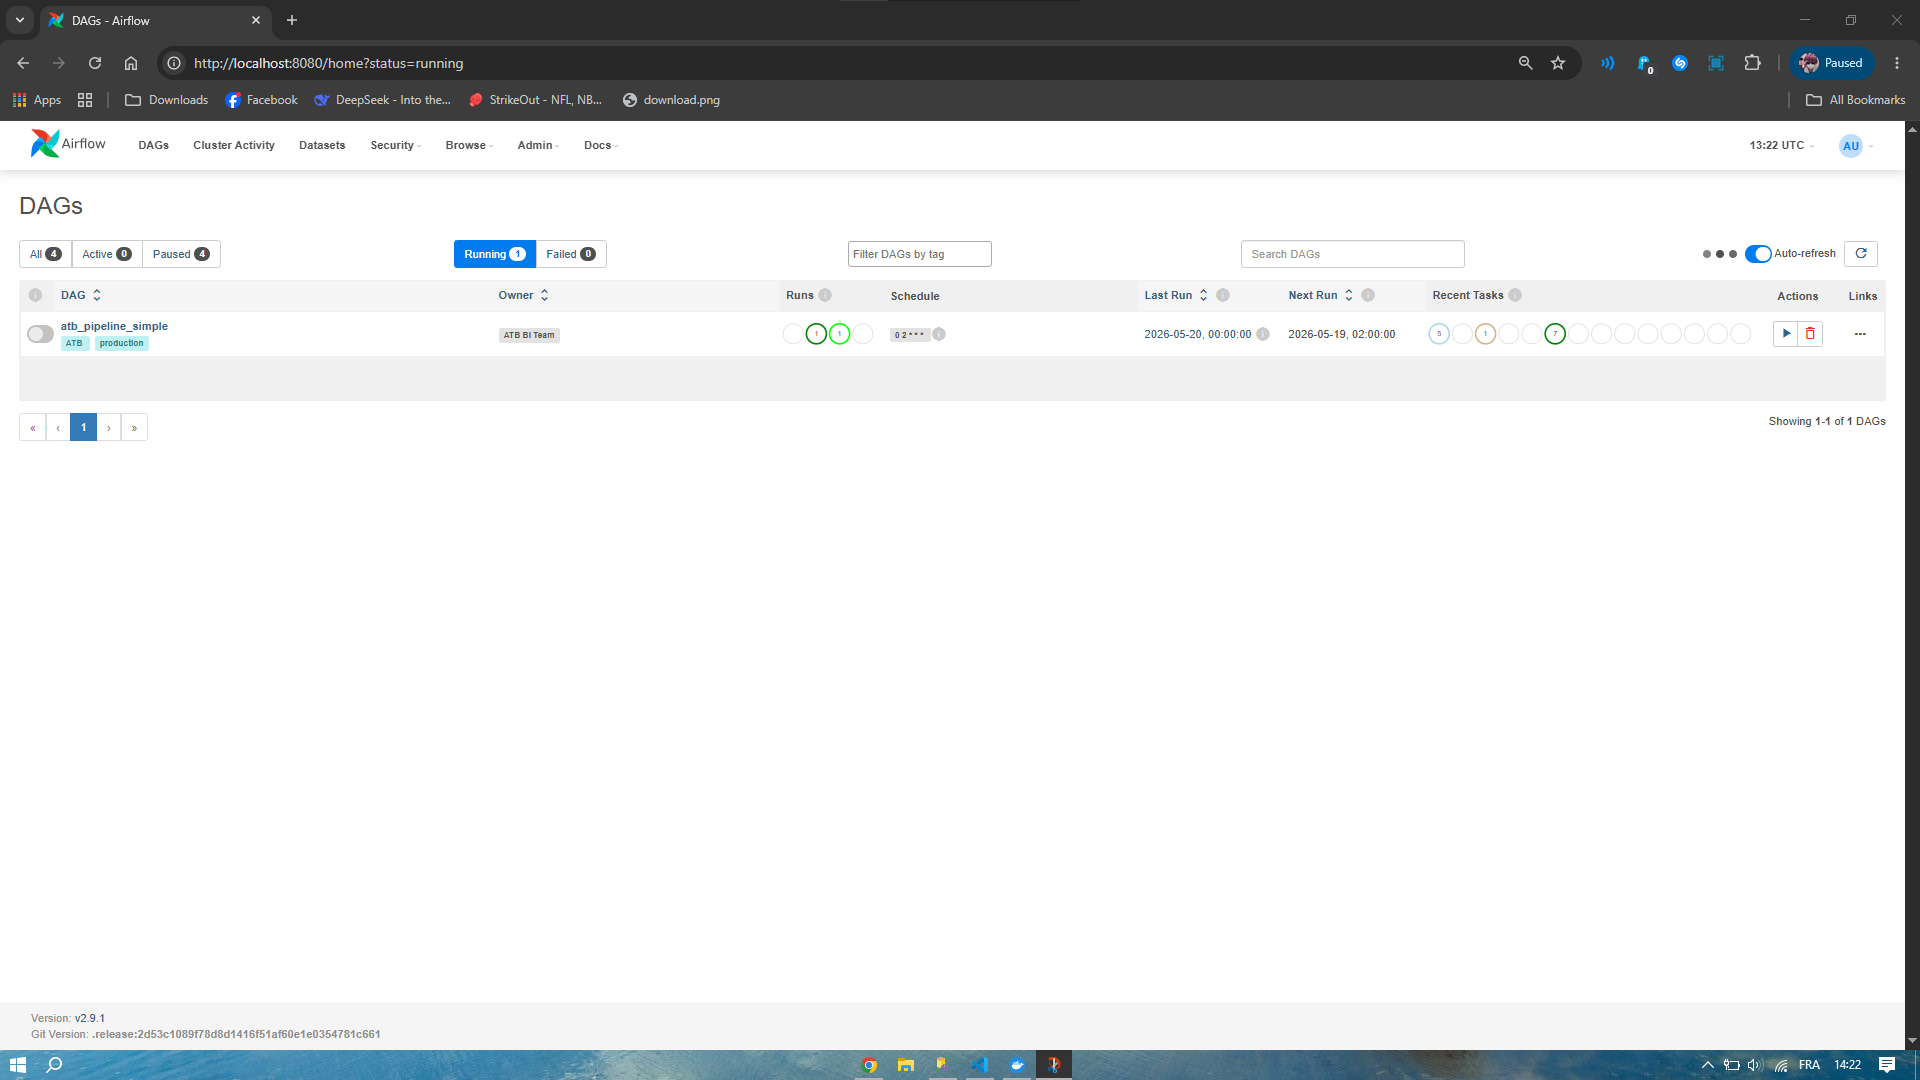
\includegraphics[width=0.88\textwidth]{figures/airflow_master_dag.png}
\caption{Airflow The machine Learning pipeline}
\label{fig:airflow-master-ml}
\end{figure}
\noindent The master DAG chains ingestion, transformation and
quality; ML retraining is gated to Sundays (or forced runs) to avoid daily cost.

The ML pipeline DAG executes three sequential tasks:
\begin{enumerate}
    \item \textbf{Train} --- runs the full model training and MLflow logging script.
    \item \textbf{Validate} --- confirms that the serialised model artefact exists and is readable.
    \item \textbf{Score} --- applies the model to all warehouse customers and persists predictions,
          including the ML probability, binary label, disagreement flag, model version, and scoring timestamp.
\end{enumerate}



% --- SCREENSHOT: Airflow UI graph view of dag_ml_pipeline
\begin{figure}[H]
\centering
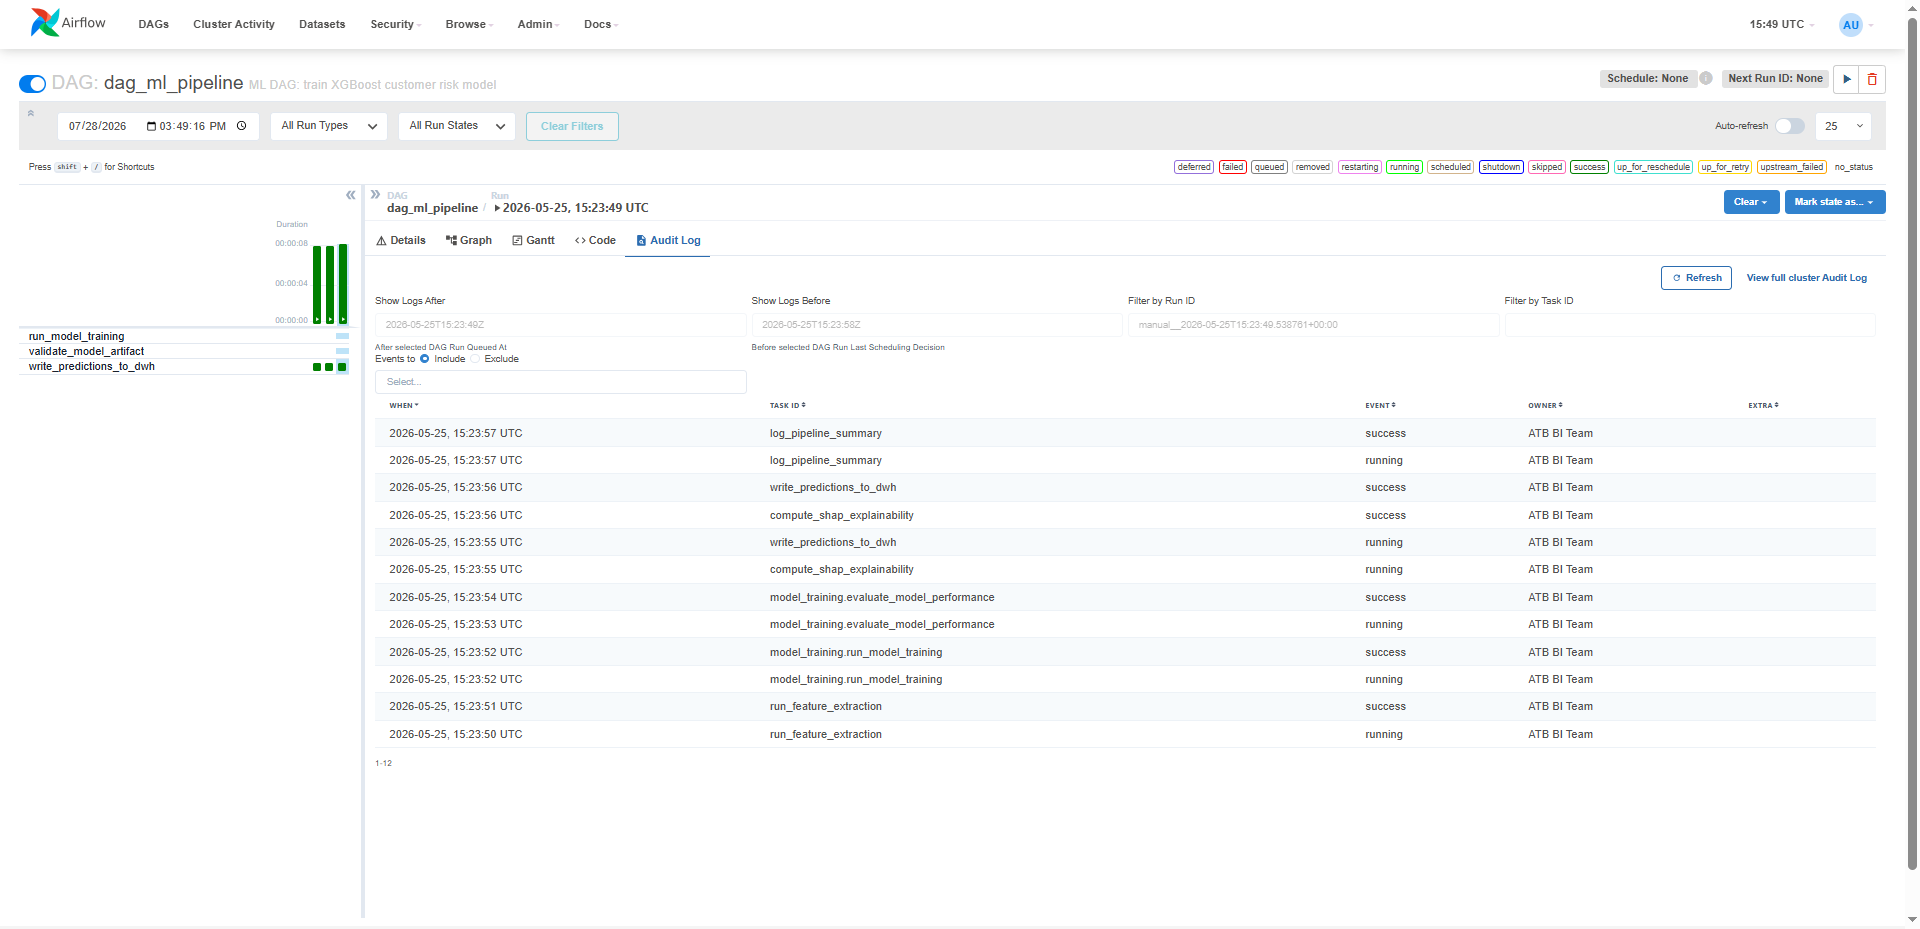
\includegraphics[width=0.90\textwidth]{figures/airflow_ml_dag.png}
\caption{Machine Learning dag graph view}
\label{fig:airflow-ml-dag}
\end{figure}
\noindent Three sequential tasks: train and log to MLflow,
validate the artefact, then batch-score the warehouse population.

% --- SCREENSHOT: SSMS showing PFE_ML.ml_customer_predictions sample rows
\begin{figure}[H]
\centering
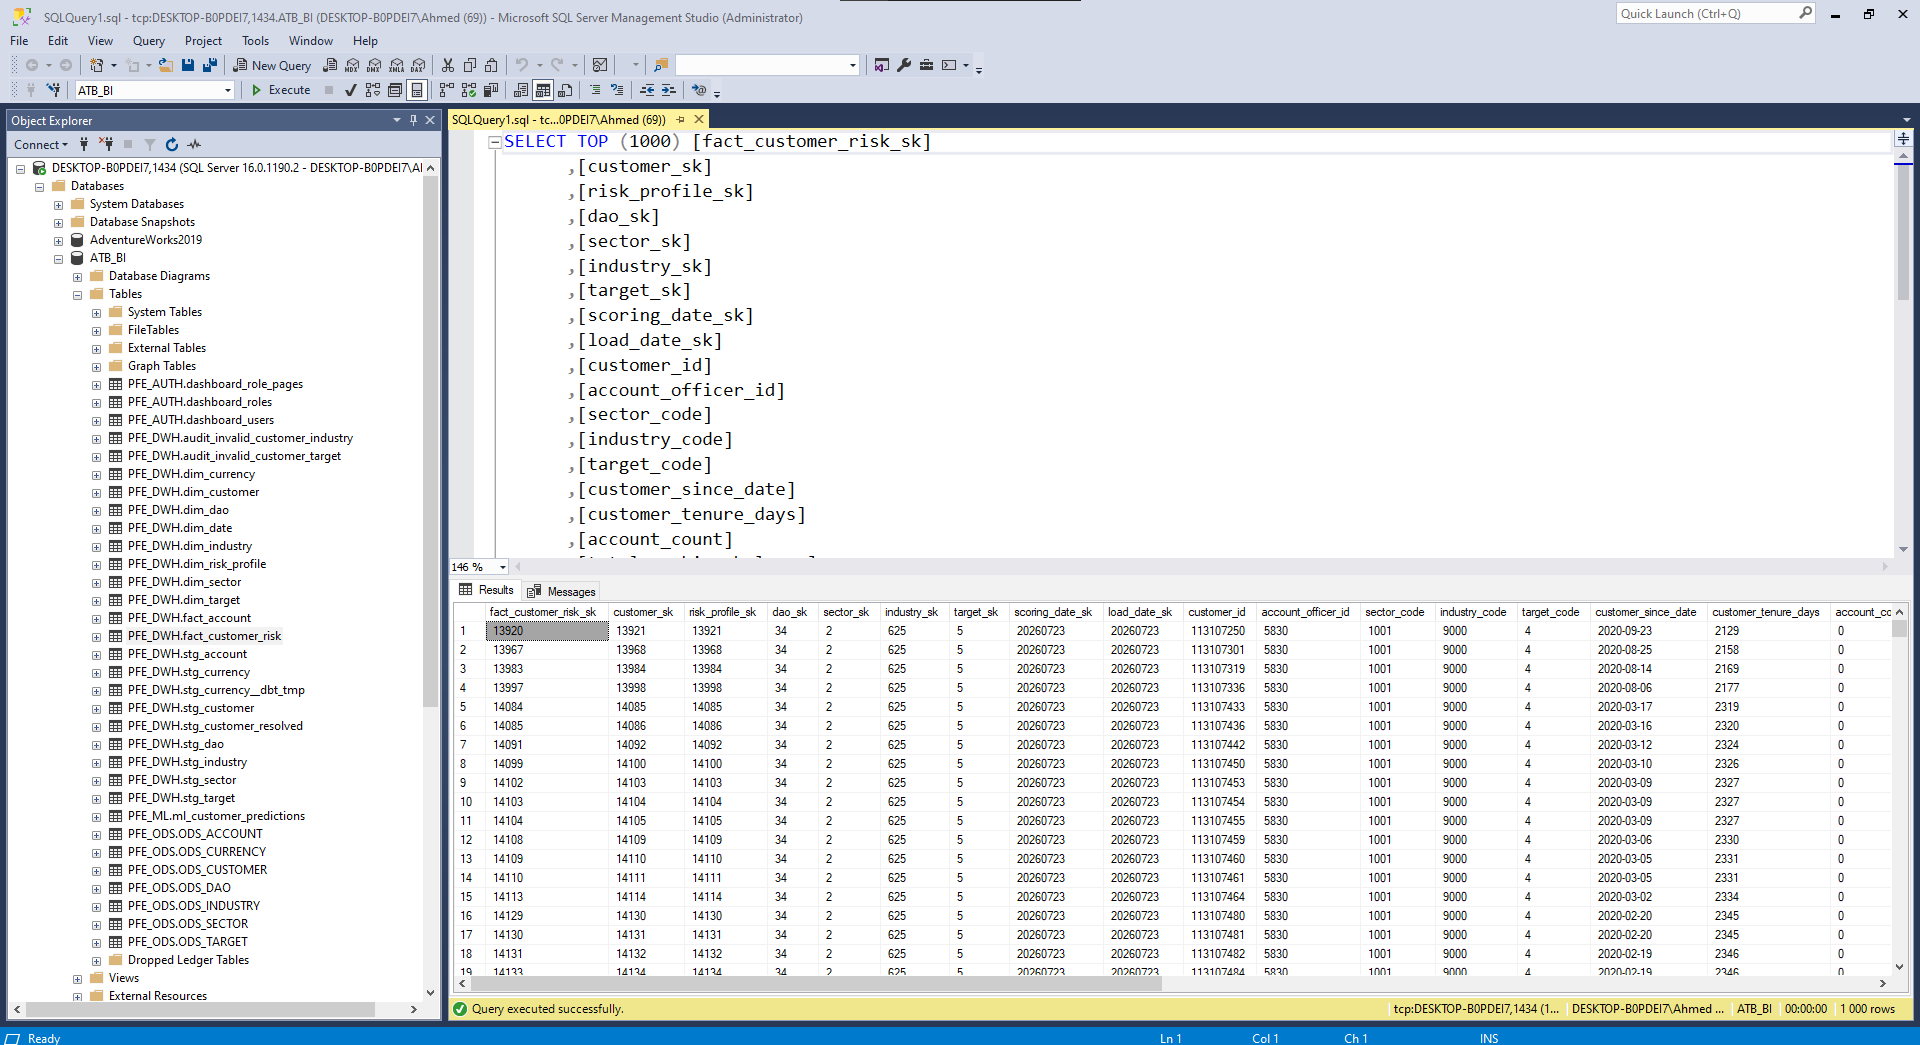
\includegraphics[width=0.90\textwidth]{figures/ssms_pfe_ml_predictions.png}
\caption{SQL Server with customer predictions filled}
\label{fig:ssms-ml-predictions}
\end{figure}
\noindent One row per customer stores probability, label,
disagreement flag, model version and scoring timestamp for the alert inbox.

\subsection{Batch Scoring Persistence}

When the ML pipeline runs, it creates the \texttt{PFE\_ML} schema if absent
and writes one row per customer into the predictions table. Each row stores
the ML risk probability, binary label, disagreement flag, model version,
and scoring timestamp, enabling the alert inbox in the dashboard to retrieve
current ML-flagged cases without re-running the model.

%======================================================================
\section{Gemini AI Integration --- Automated Chart Analysis}
\label{sec:gemini_ai}
%======================================================================

\subsection{Motivation}

A core challenge in risk management is the gap between \emph{data visibility}
and \emph{data understanding}. While a well-designed dashboard can show
compliance officers \emph{what} the numbers are --- branch risk distributions,
customer tier breakdowns, overdraft rates --- it rarely explains \emph{why}
a pattern emerges or \emph{what action} is appropriate. This gap is
particularly acute for branch managers and general management users who may
not have a quantitative background.

To address this, the ATB BI platform integrates \textbf{Google Gemini} as an
on-demand AI analyst: each chart rendered on the dashboard can be accompanied
by a concise, business-appropriate natural-language interpretation generated
automatically from the underlying data. The feature is entirely \emph{user-controlled}
--- it activates only when the user explicitly requests it, preserving
performance and privacy.

\subsection{Architecture of the AI Explanation Engine}

The explanation engine is built around \textbf{Google Gemini}
(\texttt{gemini-2.0-flash}) accessed through the official
\texttt{google-generativeai} Python SDK. The four-step pipeline is illustrated
in Figure~\ref{fig:ai-flow}:

\begin{figure}[H]
\centering
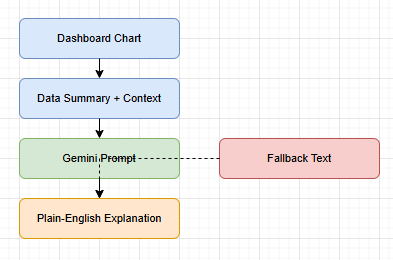
\includegraphics[width=0.62\textwidth]{figures/atb_ai_explanation_flow.png}
\caption{Gemini AI explanation pipeline}
\label{fig:ai-flow}
\end{figure}
\noindent Chart statistics become a role-aware prompt; Gemini
returns a short paragraph, or a local template keeps the panel online if the API
fails.

\begin{enumerate}
    \item \textbf{Data extraction.} When the user clicks \emph{Explain chart},
          the Streamlit page collects a statistical summary of the visible
          visualisation key metric values, dominant segments, and notable
          trends and encodes it as a structured Python dictionary.
    \item \textbf{Prompt construction.} The summary is formatted into a
          natural-language prompt that specifies the chart type, data
          dimensions, business context (ATB prudential risk dashboard), and
          the intended audience (General Management, Chief Compliance Officer,
          or Branch Manager) so that the AI response is calibrated to the
          correct level of detail.
    \item \textbf{AI inference.} The prompt is submitted to
          \texttt{gemini-2.0-flash} via \texttt{model content generator}.
          The API returns a concise, jargon-controlled paragraph tailored
          to the banking compliance domain.
    \item \textbf{Presentation and fallback.} The response is displayed inside
          an \emph{AI Analyst} expander panel directly below the chart. If
          the Gemini API is unreachable or the authentication key is not
          configured, a pre-written fallback explanation is shown, ensuring
          the dashboard is always functional regardless of API availability.
\end{enumerate}

\subsection{User Control AI Explanations Sidebar}

The \textbf{AI explanation feature is entirely opt-in and user-controlled},
reflecting a deliberate design choice: automated AI output should complement
human judgement rather than impose it. The control interface is exposed
through two mechanisms:

\begin{itemize}
    \item \textbf{Explain chart button.} Each chart panel contains an
          \emph{Explain chart} button. Pressing it triggers a single Gemini
          API call for that specific chart and renders the response
          immediately beneath it. The user can thus choose which
          visualisations they wish to have explained and which to leave
          uninterpreted.
    \item \textbf{AI Explanations sidebar section.} The left navigation panel
          of the dashboard includes a collapsible \textbf{AI explanations}
          section. Inside this section, the user can enter their personal
          \textbf{Gemini API key} directly into the interface. This allows
          each team member a branch manager in Sfax, a compliance analyst
          in Tunis to connect the AI service under their own credentials
          without any server-side configuration. If the field is left empty,
          the system operates in fallback mode with pre-authored
          interpretations, maintaining full dashboard functionality.
\end{itemize}

Figure~\ref{fig:gemini-api-studio} shows the key provisioned in
\textbf{Google AI Studio} for the project \texttt{PFE BI}
(\emph{Graph Streamlit Analyse}). Only a masked fragment of the key is
visible; the full secret is never stored in the repository and is entered
at runtime in the dashboard sidebar.

\begin{figure}[H]
\centering
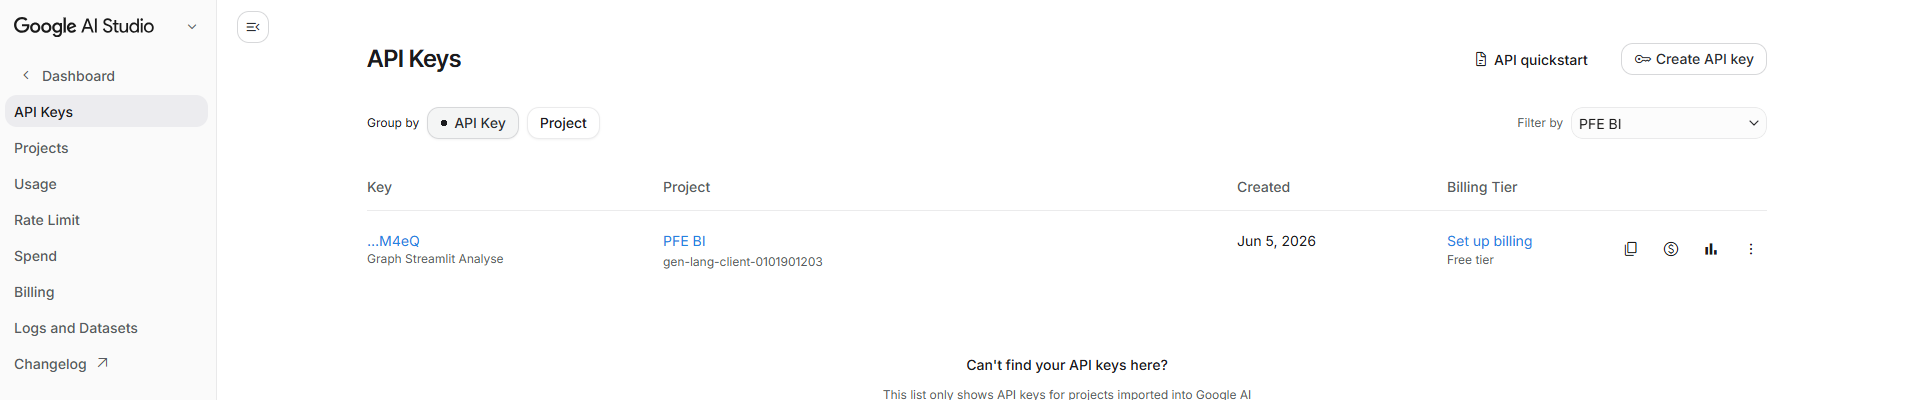
\includegraphics[width=0.92\textwidth]{figures/Google_gemni_api.png}
\caption{Google AI Studio the API key}
\label{fig:gemini-api-studio}
\end{figure}

This architecture ensures that the AI layer is \textbf{transparent},
\textbf{auditable}, and \textbf{non-blocking}: risk officers are never given
an unsolicited AI opinion, and the dashboard never fails if the AI service
is unavailable.

\subsection{Gemini AI in Practice Dashboard Examples}

Figure~\ref{fig:gemini-ai-dashboard} illustrates the AI Analyst panel in
operation on the geographic risk analysis page, which displays three
complementary visualisations simultaneously: a branch-area heatmap segmented
by risk tier, a DAO treemap, and a Tunisia bubble map. Each chart is
equipped with its own \emph{Explain chart} button. Once clicked, the
gemini model reads the data summary and produces a compliance-oriented
interpretation displayed in the right-hand panel.

\begin{figure}[H]
\centering
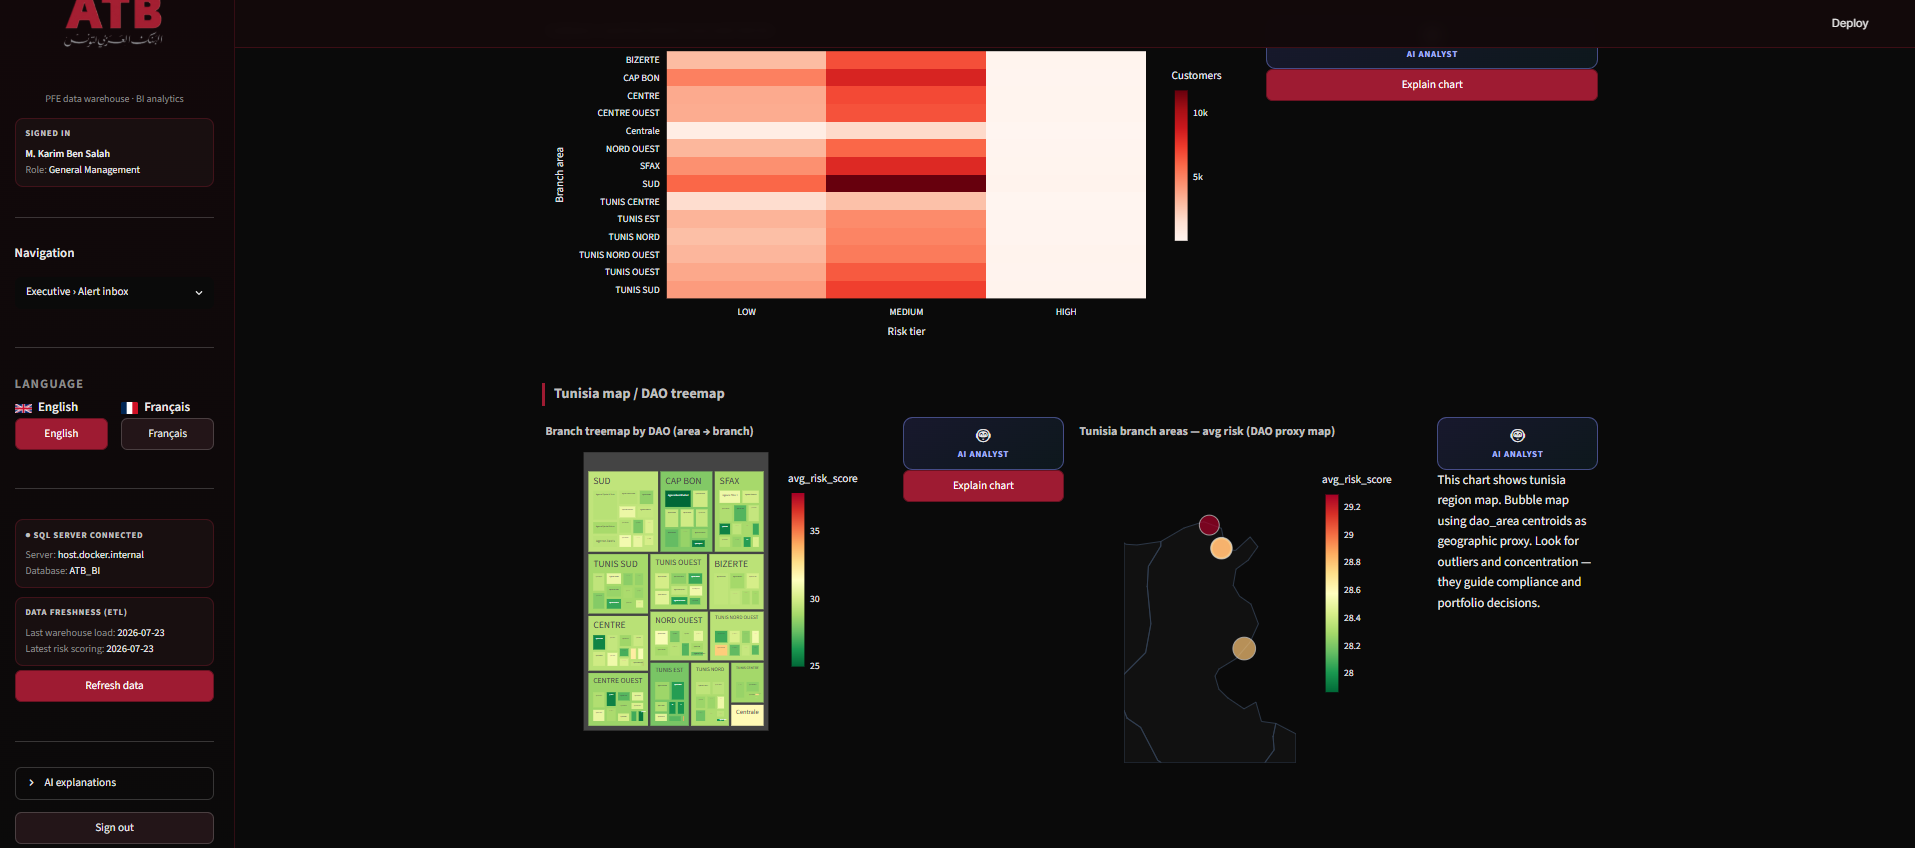
\includegraphics[width=0.95\textwidth]{figures/dash_ai_explain.png}
\caption{AI Analyst panel on-demand Gemini interpretation beside a dashboard chart}
\label{fig:gemini-ai-dashboard}
\end{figure}
\noindent Geographic risk charts (heatmap, DAO treemap, map)
each expose an Explain chart action; the response appears in the right-hand
panel without leaving the page.

\subsection{Integration with ML Outputs}

The same explanation mechanism extends to the \textbf{ML Risk Intelligence}
module, making quantitative model outputs accessible to non-technical
compliance staff:

\begin{itemize}
    \item On the \textbf{Curves \& SHAP} tab, the user can request an
          AI-generated interpretation of the probability score distribution.
          A typical response might read: ``The distribution shows that the
          vast majority of customers have a very low ML risk probability,
          consistent with the 1.3\% base rate. The right-hand tail of
          1{,}631 high-risk identifications represents the primary alert
          population that warrants compliance review.''
    \item On the \textbf{Batch \& alerts} tab, a natural-language agreement
          summary is generated on demand for example: ``The XGBoost model
          and the rules engine reach the same conclusion for 99.97\% of
          evaluated customers. The 34 remaining disagreements should be
          escalated for manual review by the compliance team.''
\end{itemize}

By combining on-demand AI narration with full user control over activation
and API credentials, the ATB BI platform establishes a responsible and
practical model of \textbf{human-in-the-loop AI governance}one where
artificial intelligence serves as a knowledgeable assistant rather than an
autonomous decision-maker.

%======================================================================
\section{Sprint 4 Summary CRISP-ML Deliverables}
\label{sec:sprint4_summary}
%======================================================================

\subsection{Deliverables by Phase}

\begin{table}[H]
\centering
\caption{Sprint~4 deliverables}
\label{tab:sprint4-deliverables-atb}
\begin{tabular}{|c|l|l|c|}
\hline
\textbf{Phase} & \textbf{Activity} & \textbf{Deliverable} & \textbf{Status} \\
\hline
1 & Business Understanding & Dual-layer rules + ML architecture & \checkmark \\
2 & Data Preparation & 5 notebooks, 34 features, SMOTETomek & \checkmark \\
3 & Model Engineering & 4 MLflow runs, XGBoost production & \checkmark \\
4 & Model Evaluation & ROC/PR, SHAP, overfitting report & \checkmark \\
5 & Deployment & ML Risk Intelligence + MLflow Registry pages & \checkmark \\
6 & Monitoring & Airflow DAGs, Docker, \texttt{PFE\_ML} scoring & \checkmark \\
\hline
\end{tabular}
\end{table}

\subsection{Production SLAs}

\begin{table}[H]
\centering
\caption{ML components in production}
\label{tab:sla-ml-production}
\begin{tabular}{|l|c|c|l|}
\hline
\textbf{Metric} & \textbf{Target} & \textbf{Result} & \textbf{Source} \\
\hline
Test F1 (XGBoost) & $\geq 0.70$ & \textbf{0.9545} & \texttt{training\_summary.json} \\
Test ROC-AUC & $\geq 0.80$ & \textbf{1.0000} & \texttt{training\_summary.json} \\
MLflow registry & Production stage & \textbf{OK} & \texttt{atb\_customer\_risk\_classifier} \\
Batch scoring table & Created & \textbf{OK} & \texttt{PFE\_ML.ml\_customer\_predictions} \\
Airflow ML DAG & Functional & \textbf{OK} & \texttt{dag\_ml\_pipeline} \\
Docker dashboard & Port 8501 & \textbf{OK} & \texttt{streamlit/Dockerfile} \\
\hline
\end{tabular}
\end{table}

%----------------------------------------------------------------------
% SCREENSHOT CHECKLIST (commented — capture these, copy to report/figures/, uncomment)
%----------------------------------------------------------------------
% ML RISK INTELLIGENCE (Streamlit ml_page.py)
%   [ ] ml_risk_intelligence_header.png   — page header + dual-layer banner + 5 tabs
%   [ ] ml_live_demo.png                  — Live demo: rules vs ML side-by-side cards
%   [ ] ml_batch_alerts.png               — Batch scoring KPIs + disagreement alert table
%   [ ] ml_curves_shap_tab.png            — ROC/PR curves + confusion matrix + SHAP
%   [ ] ml_xgboost_metrics_tab.png        — Metrics KPIs + bar charts + output gallery
%
% MLFLOW REGISTRY (Streamlit mlflow_page.py)
%   [ ] mlflow_registry_page.png          — Production card + registered models + runs
%
% JUPYTER / TRAINING OUTPUTS (copy from 4_ml/outputs/)
%   [ ] eda_target_and_distribution.png
%   [ ] eda_correlation_heatmap.png
%   [ ] 03_model_comparison_bars.png
%   [ ] 05_test_metrics_comparison.png
%   [ ] 05_roc_pr_curves.png
%   [ ] shap_local_waterfall.png
%   [ ] mlflow_dashboard.png              — optional: native MLflow UI
%
% OPS / INFRASTRUCTURE
%   [ ] airflow_ml_dag.png                — dag_ml_pipeline graph view
%   [ ] streamlit_docker_running.png
%   [ ] ssms_pfe_ml_predictions.png
%----------------------------------------------------------------------

%======================================================================
\section{Conclusion}
\label{sec:release3_conclusion}
%======================================================================

Release~3 closes the platform with a supervised learning layer aligned to CRISP-ML.
Four classifiers were compared under identical warehouse features and temporal
holdout; XGBoost was selected as the production model (test F1 $= 0.9545$,
ROC-AUC $= 1.0$) and registered in MLflow. The rules-based global risk score remains
the official auditable measure, while ML acts as a screening assistant that raises
disagreement alerts and supports what-if analysis in Streamlit.

SHAP explanations, Airflow retraining and batch scoring into \texttt{PFE\_ML} make the
model operable for compliance and risk teams without replacing the deterministic
engine. Sprint~4 therefore delivers predictive capability that is reproducible,
explainable and integrated into the same dashboard already used for BI steering.
